%-------------------------------------------------------------------------------
%
% TUM Dissertation Template
%
% For usage instructions see README.md
%
% Authors:
%   Andre Richter, andre.richter@tum.de
%   Michael Vonbun, michael.vonbun@tum.de
%   Christian Herber, christian.herber@tum.de
%   Stefan Wallentowitz, stefan.wallentowitz@tum.de
%
%-------------------------------------------------------------------------------
\documentclass[%
  % layouttitlepage,            % layout help rules (to see if you need
  %                             % some extra vspace in your title etc.)
  % headings = standardclasses, % serif fonts for headings
  % headings = big,             % If you use serif fonts for headings (above option
  %                             % uncommmented), uncomment this one to get smaller
  %                             % headings
  % sansseriftitlepage,         % sans serif title page
  % notocintoc,                 % do not add toc to toc itself
]{tumDiss}
\usepackage[utf8]{inputenc}

%-------------------------------------------------------------------------------
% Binding correction for the title page.
% WARNING: ONLY NEEDED FOR THE PRINT VERSION!
%
% After printing and binding, the left part of the titlepage may lose
% significant space, for example due to overlap from glue binding.
% You can increase the left margin of the title page with this option.
% This value of 8mm was measured for glue binding a thesis that was printed by
% the TUM Fachschaft EI and ~140 pages.
%-------------------------------------------------------------------------------
% \titlepagebindingcor{8mm}

%-------------------------------------------------------------------------------
% Binding correction for everything else.
% Does not affect titlePageBindingCor!
%
% WARNING: THIS OPTION CAN SHAKE UP YOUR CURRENT LAYOUT.
% If you want to use it, it is best to work with it from the very start. Adding
% it when finishing your dissertation might get you into trouble.
%
% Search http://texdoc.net/texmf-dist/doc/latex/koma-script/scrguien.pdf for
% "BCOR" for further reading.
%-------------------------------------------------------------------------------
% \KOMAoptions{BCOR=3mm}

%-------------------------------------------------------------------------------
% Faculty
%-------------------------------------------------------------------------------
\faculty{TUM School of Medicine and Health}

%-------------------------------------------------------------------------------
% Degree
%-------------------------------------------------------------------------------
\degree{Doktors der Naturwissenschaften\\(Dr. rer.\ nat.)}

%-------------------------------------------------------------------------------
% Title
%
% IMPORTANT:
%
% You must add manual line breaks here. If you don't, you'll get uneven spacing
% between the lines.
% YOU ALSO NEED THE BREAK AT THE LAST LINE.
%-------------------------------------------------------------------------------
\title{Deep Clustering of Animal Motion Tracking Data: \\ }
\subtitle{software development and applications to \\ psychiatric preclinical research}

%-------------------------------------------------------------------------------
% People
%-------------------------------------------------------------------------------
\author{Lucas Miranda}
\vorsitz{ }
\erstpruef{Prof.\ Dr.\ Bertram Müller-Myhsok}

% Use this one for a TUM professor
% \zweitpruef{Prof. Dr.-Ing. Vorname Nachname}

% Or this one for an external professor
\zweitpruef{Prof.\ Dr.\ Julien Gagneur}

% Optionally, add a third examiner
%\drittpruef[RWTH Aachen]{Prof. Dr.-Ing. Max Mustermann}

%-------------------------------------------------------------------------------
% Hand in date
%
% This is the date of your personal hand-in at the TUM doctoral office.
%-------------------------------------------------------------------------------
\date{18.07.2023}

%-------------------------------------------------------------------------------
% Accepted date
%
% You can set this after your thesis was accepted. For handing in,
% it is not needed (at least for the Electrical Engineering faculty).
%-------------------------------------------------------------------------------
\dateaccepted{08.11.2023}



%-------------------------------------------------------------------------------
% Change language, e.g. to german
%-------------------------------------------------------------------------------
\usepackage[main=english, german]{babel}

%-------------------------------------------------------------------------------
% Compatibility issues
%-------------------------------------------------------------------------------
% If you need pstricks, load it here before everything else.
% Otherwise, tikz patterns won't work
%\usepackage{pstricks}

%-------------------------------------------------------------------------------
% Suggested standard packets are included here
%-------------------------------------------------------------------------------
% Loading scrhack fixes:
%   (1) KOMA-Script incompatible macros used in listings package.
%   (2) Inconsistent anchors in hyperref.
\usepackage{scrhack}


% figure inclusion
\usepackage[
  caption = false,
  font    = footnotesize
]{subfig}
\usepackage{graphicx}
\usepackage{pgfplots}
\usepackage{pgfplotstable}
\tikzset{>=stealth}
\usetikzlibrary{patterns}
\usetikzlibrary{pgfplots.statistics}

% code block insertion
\usepackage{moreverb}
\usepackage{listings}

% math and equations
\usepackage{amsmath}
\usepackage{amssymb}
\usepackage{amsfonts}
\usepackage{upgreek}

\expandafter\def\expandafter\normalsize\expandafter{%
  \normalsize  
  \setlength\abovedisplayskip{4ex}
  \setlength\belowdisplayskip{4ex}
  \setlength\abovedisplayshortskip{4ex}
  \setlength\belowdisplayshortskip{4ex}
}

% enumeration
\usepackage{enumerate}

% Source code with highlighting
\usepackage{listings}
\lstset{
  basicstyle       = \footnotesize,
  captionpos       = b,
  tabsize          = 4,
  commentstyle     = \color{TUMGreen},
  keywordstyle     = \color{TUMBlue},
  stringstyle      = \color{TUMOrange},
  otherkeywords    = {
    uint64_t,
    uint32_t,
    uint16_t,
    uint8_t,
    u64,
    u32,
    u16,
    u8,
    inline
  },
  numbers          = left,
  xleftmargin      = 7ex,
  aboveskip        = 4ex,
  abovecaptionskip = 2ex,
}

% Support for siunitx
\usepackage{siunitx}
\sisetup{
  exponent-product = \cdot,
  output-product   = \cdot,
  per-mode         = symbol-or-fraction,
  quotient-mode    = fraction,
  binary-units     = true
}

% No widows and orphans
\usepackage[all]{nowidow}

% dummy text
\usepackage{pdfpages}
\usepackage{float}

% hyperlinks
% according to its documentation, hyperref should be loaded last
% a list of packages that should be loaded after hyperref can be found at
% https://tex.stackexchange.com/questions/1863/which-packages-should-be-loaded-after-hyperref-instead-of-before
\usepackage{url}
\usepackage[
  hidelinks,
  bookmarksnumbered,
  breaklinks,
]{hyperref}

% If hyperref is used, references to tables and figures link to their captions
% and not the actual tables or figures. This is especially unwanted for figures,
% because their captions are below the figure so that clicking on a link just
% shows the captions and the figure is invisible.
%
% Using the caption package fixes this behaviour.
\usepackage{caption}

% glossary functionality
% loading glossaries after hyperref adds hyperlings to acronyms and glossary
% entries
\usepackage[
  toc,
  acronym,
  style = long
]{glossaries}
\makeglossaries

%-------------------------------------------------------------------------------
% Include custom packages here
%-------------------------------------------------------------------------------

\usepackage[resetlabels,labeled]{multibib}
\newcites{PhD}{List of published PhD papers}

%-------------------------------------------------------------------------------
% TUM CI colors for PGF
%-------------------------------------------------------------------------------
\definecolor{grey60} {RGB} {102, 102, 102} % 60% grey

%-------------------------------------------------------------------------------
% Default values for pgfplots
%-------------------------------------------------------------------------------
\newcommand{\figureHeight}{0.5625} %% 16:9
\pgfplotsset{
  compat           = 1.13,
  grid             = major,
  enlarge x limits = 0,
  cycle list name  = tum,
  major grid style = {dotted},
  minor grid style = {dotted},
  legend style     = {
    at     = {(0.98,0.96)},
    anchor = north east,
  },
  width            = \hsize * 0.9,
  height           = \hsize * 0.9 * \figureHeight,
}

%-------------------------------------------------------------------------------
% Correct bad hyphenation here
%-------------------------------------------------------------------------------
\hyphenation{op-tical net-works semi-conduc-tor}

%-------------------------------------------------------------------------------
% Acronyms (will be sorted alphabetically)
%-------------------------------------------------------------------------------
\newacronym{csds}{CSDS}{Chronic Social Defeat Stress}
\glsadd{csds}

\newacronym{shap}{SHAP}{SHapley Additive exPlanations}
\glsadd{shap}

\newacronym{vade}{VaDE}{Variational Deep Embeddings}
\glsadd{vade}

\newacronym{vae}{VAE}{Variational AutoEncoder}
\glsadd{vae}

\newacronym{vqvae}{VQVAE}{Vector Quantization Variational AutoEncoder}
\glsadd{vqvae}

\newacronym{rnn}{RNN}{Recurrent Neural Network}
\glsadd{rnn}

\newacronym{tcn}{TCN}{Temporal Convolutional Network}
\glsadd{tcn}

\newacronym{si}{SI}{Social Interaction}
\glsadd{si}

\newacronym{sa}{SA}{Social Avoidance}
\glsadd{sa}

\newacronym{of}{OF}{Open Field}
\glsadd{of}

\newacronym{gnn}{GNN}{Graph Neural Network}
\glsadd{gnn}

\newacronym{gmm}{GMM}{Gausian Mixture Model}
\glsadd{gmm}

\newacronym{dlc}{DLC}{DeepLabCut}
\glsadd{dlc}

\newacronym{mdd}{MDD}{Major Depressive Disorder}
\glsadd{mdd}

\newacronym{ptsd}{PTSD}{Post-Traumatic Stress Disorder}
\glsadd{ptsd}

\newacronym{mri}{MRI}{Magnetic Resonance Imaging}
\glsadd{mri}

\newacronym{fmri}{fMRI}{functional Magnetic Resonance Imaging}
\glsadd{fmri}

\newacronym{vame}{VAME}{Variational Animal Motion Embeddings}
\glsadd{vame}

\newacronym{sleap}{SLEAP}{Social LEAP Estimates Animal Poses}
\glsadd{sleap}

\newacronym{dls}{DLS}{Depressive-like Syndrome}
\glsadd{dls}

\newacronym{rdoc}{RDoC}{Research Domain Criteria}
\glsadd{rdoc}

\newacronym{icd}{ICD}{International Classification of Diseases}
\glsadd{icd}

\newacronym{ann}{ANN}{Artificial Neural Network}
\glsadd{ann}

\newacronym{dnn}{DNN}{Deep Neural Network}
\glsadd{dnn}

\newacronym{ai}{AI}{Artificial Intelligence}
\glsadd{ai}

\newacronym{gan}{GAN}{Generative Adversarial Network}
\glsadd{gan}

\newacronym{rcnn}{R-CNN}{Region-based Convolutional Neural Network}
\glsadd{rcnn}

\newacronym{knn}{KNN}{K-Nearest Neighbors}
\glsadd{knn}

\newacronym{rfid}{RFID}{Radio-frequency identifier}
\glsadd{rfid}

\newacronym{gbm}{GBM}{Gradient Boosting Machine}
\glsadd{gbm}

\newacronym{vr}{VR}{Virtual Reality}
\glsadd{vr}

\newacronym{hpa}{HPA axis}{Hypothalamic-Pituitary-Adrenal axis}
\glsadd{hpa}

\newacronym{sns}{SNS}{Sympathetic Nervous System}
\glsadd{sns}

\newacronym{dtw}{DTW}{Dynamic Time Warping}
\glsadd{dtw}

\newacronym{hmm}{HMM}{Hidden Markov Model}
\glsadd{hmm}

\newacronym{arhmm}{AR-HMM}{Autoregressive Hidden Markov Model}
\glsadd{arhmm}

\newacronym{dbscan}{DBSCAN}{Density-based spatial clustering of applications with noise}
\glsadd{dbscan}

\newacronym{hdbscan}{HDBSCAN}{Hierarchical Density-based spatial clustering of applications with noise}
\glsadd{hdbscan}

\newacronym{tsfresh}{tsfresh}{Time Series FeatuRe Extraction on basis of Scalable Hypothesis tests}
\glsadd{tsfresh}

\newacronym{pca}{PCA}{Principal Component Analysis}
\glsadd{pca}

\newacronym{umap}{UMAP}{Uniform Manifold Approximation and Projection}
\glsadd{umap}

\newacronym{fps}{FPS}{Frames Per Second}
\glsadd{fps}

\newacronym{joss}{JOSS}{Journal of Open Source Software}
\glsadd{joss}

\newacronym{deepof}{DeepOF}{Deep Open Field}
\glsadd{deepof}

\newacronym{ci}{CI}{Continuous Integration}
\glsadd{ci}

\newacronym{stgnn}{ST-GNN}{Spatio-Temporal Graph Neural Network}
\glsadd{stgnn}

\newacronym{kld}{KLD}{Kullback-Leibler Divergence}
\glsadd{kld}

\newacronym{elbo}{ELBO}{Evidence Lower Bound}
\glsadd{elbo}

\newacronym{crl}{CRL}{Contrastive Representation Learning}
\glsadd{crl}

\newacronym{nce}{NCE}{Noise Contrastive Estimation}
\glsadd{nce}

\newacronym{llm}{LLM}{Large Language Model}
\glsadd{llm}

\newacronym{ml}{ML}{Machine Learning}
\glsadd{ml}

\newacronym{qtl}{QTL}{Quantitative Trait Loci}
\glsadd{qtl}

% BP marginpar
\newcommand{\bpmp}[1]{\marginpar{{\tiny BP: #1}}}
\newcommand{\python}[1]{{\texttt{#1}}}
\newcommand{\cref}[1]{chapter~\ref{#1}}
\newcommand{\Cref}[1]{Chapter~\ref{#1}}
\newcommand{\Sim}{\mathrm{Sim}}
\newcommand{\josstitle}{\textbf{``DeepOF: a Python package for supervised and unsupervised pattern recognition in mice motion tracking data"}}
\newcommand{\natcommtitle}{\textbf{``Automatically annotated motion tracking identifies a distinct social behavioral profile following chronic social defeat stress"}}
\newcommand{\fullncref}{can be retrieved from the publication \natcommtitle, included as part of \cref{chap:natcomm}}
%-------------------------------------------------------------------------------
% Actual document starts here
%-------------------------------------------------------------------------------
\begin{document}
\frontmatter
\maketitle

%-------------------------------------------------------------------------------
\chapter{Acknowledgements}
\hspace{0pt}
\vfill

\begin{center}

\textit{To Tomás}\\
\textit{To Sol}\\
\textit{To Pedro}\\
\textit{To Tamayo, Stella, Olga, and Tito}\\
\textit{To Flor}\\
\textit{To Fabio and Silvina}\\
\textit{who told me the sky was the limit}\\
\textit{and taught me how to fly}\\

\end{center}

\begin{figure}[!thb]
\centering
\includegraphics[width=250pt]{Figures/acknowledgements_1.pdf}
\centering
\vfill
\end{figure}

\vfill
\hspace{0pt}

\newpage

The work presented here would not have been possible without the help and support of Benno Pütz (my great mentor and travel companion), Joeri Bordes (whose hard work and contributions were invaluable in conceiving and implementing DeepOF and its applications), Mathias V. Schmidt, and, of course, Bertram, who let me make my own path and explore interdisciplinary collaborations, while always being there for me.

Along these lines, I feel the need to highlight the beautiful collaborative atmosphere within the Max Planck Institute of Psychiatry and the International Max Planck Research School for Translational Psychiatry (IMPRS-TP). Most (if not all) of my work was sparked by interactions with other research groups within these institutions, where complementary expertise and the learning of a common language were (and continue to be) key to reaching our humble goals. Special thanks to Darina Czamara and Juan Pablo Lopez, who supported me with advice and presented me with opportunities at all times, and to Elisabeth Binder.

On top of this, I was fortunate enough to have been part of the Machine Learning Frontiers in Precision Medicine Marie Curie Innovative Training Network (MLFPM-ITN). Here, people like Felix Agakov, Karsten Borgwardt, Katharina Heinrich, and many others, made sure I and all students had everything we needed to thrive in our own individual and collective scientific endeavors. For this I am immensely grateful.

Last but not least, I thank my friends and family back home. Their unconditional support, love, and company in the distance were key to finding motivation, especially through the difficult times many of us endured in isolation over the last couple of years.

%-------------------------------------------------------------------------------
\chapter{Abstract}
% Definition of behavior
Attempts to systematically characterize and understand how living organisms react to complex stimuli are not new. Until recently, however, most approaches have either relied on observational studies, which prevent researchers from testing specific hypotheses, or in overly simplified and laborious laboratory settings, that are too far from real-world scenarios. Along these lines, a recent trend has been to recreate semi-naturalistic scenarios in a controlled manner, and use new technologies to extract information from freely moving animals such as motion tracking, neural activity, and vocalization, among others.

% DeepLabcut and motion tracking
In the field of motion tracking, and leveraging advances in machine learning, particularly in neural networks used for computer vision, several openly available software packages have recently started to provide tools that require little effort to accurately track multiple body parts over time, without the need for physical markers. This has opened the way for researchers to obtain large amounts of data with little effort, which has in turn helped developers come up with novel ways to analyze and extract insight from this novel data source.

% Three  main goals
Thus and so, the current thesis aims to provide three main contributions. First, to develop novel deep clustering algorithms specifically tailored to this type of time series, that can be used to explore the behavioral repertoire of animals without the need of human labels. Second, the deployment of these algorithms in an open-source Python package, which includes them alongside other tools to annotate the behavior of laboratory rodents. Third and last, to use the deployed algorithms to characterize a real world animal model.

% Introducing DeepOF
Moreover, this is a publication-based dissertation, which presents the accomplished results as two papers accepted for publication in peer-reviewed journals. The first two mentioned goals are addressed in an article published in the Journal of Open Source Software (JOSS), titled \josstitle. Here, we present an originally developed software tool called DeepOF (Deep Open Field), which includes several deep clustering algorithms alongside other tools, and is ready for researchers to use. 

% Introducing CSDS
The second paper was published in Nature Communications, and is titled \natcommtitle. Here, we present a characterization of Chronic Social Defeat Stress (CSDS), an animal model widely used in stress and depression research, using the novel software presented in the first article.

% Closing remarks
All in all, this thesis provides a set of novel contributions to both the behavioral research field in general, and the analysis of motion tracking data in particular. The next few chapters will describe these contributions in detail, and how I believe they hold the potential to positively impact future research.


%-------------------------------------------------------------------------------
\chapter{Zusammenfassung}
\begin{otherlanguage}{german}

% Definition von Verhalten
Versuche, systematisch zu charakterisieren und zu verstehen, wie lebende Organismen auf komplexe Reize reagieren, sind nicht neu. Bis vor kurzem stützten sich die meisten Ansätze jedoch entweder auf Beobachtungsstudien, die es den Forschern unmöglich machen, spezifische Hypothesen zu testen, oder auf allzu vereinfachte und mühsame Laborsituationen, die zu weit von realen Szenarien entfernt sind. In diesem Sinne geht der Trend in letzter Zeit dahin, halbnatürliche Szenarien kontrolliert nachzustellen und neue Technologien einzusetzen, um Informationen von sich frei bewegenden Tieren zu extrahieren, wie z.B. Bewegungsverfolgung, neuronale Aktivität und Vokalisierung.

% DeepLabcut und Bewegungsverfolgung
Auf dem Gebiet der Bewegungsverfolgung und unter Ausnutzung der Fortschritte im Bereich des maschinellen Lernens, insbesondere bei neuronalen Netzen, die für das Computersehen verwendet werden, haben mehrere frei verfügbare Softwarepakete in letzter Zeit begonnen, Tools bereitzustellen, die mit geringem Aufwand eine genaue Verfolgung mehrerer Körperteile über die Zeit ermöglichen, ohne dass physische Marker erforderlich sind. Dies hat Forschern die Möglichkeit eröffnet, mit geringem Aufwand große Datenmengen zu erhalten, was wiederum Entwicklern geholfen hat, neue Wege zu finden, um diese neuartige Datenquelle zu analysieren und Erkenntnisse daraus zu gewinnen.

% Drei Hauptziele
Die vorliegende Arbeit zielt also darauf ab, drei Hauptbeiträge zu leisten. Erstens die Entwicklung neuartiger Deep Clustering-Algorithmen, die speziell auf diese Art von Zeitreihen zugeschnitten sind und mit denen sich das Verhaltensrepertoire von Tieren ohne menschliche Kennzeichnung erforschen lässt. Zweitens, die Bereitstellung dieser Algorithmen in einem Open-Source-Python-Paket, das sie zusammen mit anderen Tools zur Annotation des Verhaltens von Labornagern enthält. Drittens und letztens, die Verwendung der eingesetzten Algorithmen zur Charakterisierung eines realen Tiermodells.

% Einführung in DeepOF
Darüber hinaus handelt es sich um eine publikationsbasierte Dissertation, in der die erzielten Ergebnisse in Form von zwei zur Veröffentlichung in begutachteten Fachzeitschriften angenommenen Artikeln präsentiert werden. Die ersten beiden genannten Ziele werden in einem im Journal of Open Source Software (JOSS) veröffentlichten Artikel mit dem Titel \josstitle behandelt. Hier stellen wir ein ursprünglich entwickeltes Software-Tool namens DeepOF (Deep Open Field) vor, das neben anderen Tools auch mehrere Deep-Clustering-Algorithmen enthält und für Forscher einsatzbereit ist. 

% Einführung in CSDS
Die zweite Arbeit wurde in Nature Communications veröffentlicht und trägt den Titel \natcommtitle. Hier stellen wir eine Charakterisierung von Chronic Social Defeat Stress (CSDS) vor, einem in der Stress- und Depressionsforschung weit verbreiteten Tiermodell, bei dem die im ersten Artikel vorgestellte neue Software zum Einsatz kommt.

% Schlussbemerkungen
Alles in allem liefert diese Arbeit eine Reihe neuartiger Beiträge sowohl zur Verhaltensforschung im Allgemeinen als auch zur Analyse von Motion-Tracking-Daten im Besonderen. In den nächsten Kapiteln werden diese Beiträge im Detail beschrieben und wie ich glaube, dass sie das Potenzial haben, die zukünftige Forschung positiv zu beeinflussen.

\end{otherlanguage}

%-------------------------------------------------------------------------------

\tableofcontents
\listoffigures
\listoftables

\printglossary[type=\acronymtype, nonumberlist]

%-------------------------------------------------------------------------------
\mainmatter
\chapter{Introduction}
\label{chap:introduction}
\section{Clinical and preclinical research: altered behavior in psychiatric conditions}

\subsection{Defining behavior}

Behavior is a fascinating and complex phenomenon which lies at the core of our existence as living organisms. The term refers to the manifestation of an individual's actions and reactions in response to external or internal stimuli, ultimately shaping interactions with the environment and other living things. Our understanding of behavior has evolved over time, and from a biological perspective, it encompasses an intricate interplay between genetic, neurobiological, and physiological processes \cite{Levitis2009BehaviouralBehaviour}.

To fully grasp the concept of behavior, it is essential to recognize the diverse nature of biological systems involved in its regulation. At the genetic level, heredity and individual variations in genetic makeup play a crucial role in shaping behavioral traits \cite{Charney2017GenesGenetics}. Genes can influence behavior through the expression of specific proteins, which in turn participate in the development, structure, and function of the nervous system \cite{Zhou2021Gene-EnvironmentPerspective}. While it is important to consider the impact of genetic factors, it is also necessary to acknowledge the interaction between genetics and environmental influences on behavior. This interplay, referred to as gene-environment interaction, highlights the dynamic nature of behavior and the continuous adaptation of living organisms to their surroundings \cite{Cuevas2019NeurotransmittersCycle}.

Moreover, a central component of behavior is the nervous system, responsible for receiving, processing, and transmitting information. It constitutes a highly organized network of specialized cells, such as neurons, which communicate with one another through complex electrochemical signaling, allowing for the integration and processing of sensory inputs, generation of responses, and modulation of behavior. Along these lines, neurotransmitters, the chemical messengers facilitating communication between neurons, also play a vital role in the regulation of behavior. These molecules, released by neurons, bind to specific receptors on the receiving cell, initiating a cascade of events that may either excite or inhibit the cell \cite{Luo2020PrinciplesNeurobiology}. 

Furthermore, another critical aspect of behavior is the interplay between the nervous and the endocrine systems. The latter is responsible for the production and release of hormones: chemical messengers secreted by endocrine glands that travel through the bloodstream and exert their effects on target cells \cite{Gardner2017GreenspansEdition}. Hormones can influence behavior by acting on the brain and other tissues, modulating emotions, mood, and stress responses \cite{McEwen2020HormonesScience}. Examples of hormones with significant impact on behavior include cortisol, which is involved in the stress response \cite{OConnor2020StressRisk}, and oxytocin, which plays a role in social bonding and attachment \cite{Bosch2018OxytocinDisruption}.

All in all, the delicate balance of neurotransmitters such as dopamine, serotonin, and glutamate, and hormones such as those mentioned above, is essential for maintaining normal behavioral functions. Disruptions in this balance can thus result in altered behavior, as seen in various psychiatric disorders \cite{AmericanPsychiatricAssociation2022DiagnosticDisorders}.

\subsection{A brief history of psychiatry}

The study of these altered behaviors, encompassed by the field of psychiatry, has a rich and storied history, marked by evolving theories and approaches to understanding and treating altered behavior in the context of mental health. The beginnings of psychiatry can be traced back to ancient civilizations, where mental disorders were often attributed to supernatural forces or divine intervention \cite{Fornaro2009MedicinePrejudices}. However, the modern understanding of psychiatry truly emerged during the Age of Enlightenment in the 18th century, when the focus shifted towards a more scientific and humane approach to mental health \cite{Kendler2022The1650-1850}.

One of the pioneers of this era was Philippe Pinel, a French physician who advocated for a compassionate approach to treating individuals with mental disorders. He emphasized the importance of understanding the root causes of altered behavior, paving the way for the development of modern psychiatric theories and therapies \cite{Wallace2008HistoryPsychology}. As psychiatry evolved throughout more recent periods of history, the field expanded its knowledge of the underlying biological processes influencing behavior, drawing upon the aforementioned discoveries in genetics, neurobiology, and endocrinology.

The 20th century marked significant advances in psychiatric research and treatment, driven by the emergence of psychoanalysis, behaviorism, and psychopharmacology. Sigmund Freud's psychoanalytic theory, which focused on unconscious processes and internal conflicts, had a profound impact on the understanding of human behavior \cite{Pick2015Psychoanalysis:Introduction}. Simultaneously, behaviorism, led by figures such as John Watson and B.\,F. Skinner, emphasized the role of observable behaviors and environmental influences in shaping human behavior \cite{Holland1978Behaviorism:Solution}. Psychopharmacology, the study of how drugs affect the mind and behavior, opened new avenues for treating psychiatric disorders by targeting the imbalances in neurotransmitters and hormones associated with them \cite{Rothschild2022Psychopharmacology:Basics}.

Despite the progress made in understanding and treating psychiatric disorders throughout history, however, challenges remain in fully elucidating the complex biological processes underlying altered behavior \cite{Harmer2017HowApproaches}. To address these challenges, researchers have increasingly turned to animal models as invaluable tools for studying the genetic, neurobiological, and physiological aspects of behavior \cite{Winship2019AnSchizophrenia, Varghese2017AutismModels, Wang2017TheDepression, Campos2013AnimalStress, Richter-Levin2019AnimalMet}. These models provide controlled environments in which researchers can manipulate specific factors, such as genetic mutations or environmental stressors, and measure their impact, typically in specific relevant variables \cite{Baker2020RodentPromises}.

Animal research has thus yielded essential insights into the neurobiology of psychiatric disorders, such as the role of neurotransmitter systems, neural circuitry, and genetic factors in the manifestation of altered behavior. For instance, rodent models have been crucial in understanding the role of dopamine in reward-related behaviors and addiction \cite{Wise2021DopamineAddiction}, as well as the involvement of serotonin in mood regulation and the pathophysiology of depression \cite{Borroto-Escuela2021TheProspects}. Additionally, animal models of stress have helped to elucidate the biological underpinnings of stress-related psychiatric disorders, such as anxiety and post-traumatic stress disorder (PTSD) \cite{Campos2013AnimalStress, Richter-Levin2019AnimalMet}. These findings highlight the importance of accurate behavioral quantification in understanding the etiology and progression of psychiatric disorders, as well as in the development of novel therapeutic strategies.

\subsection{Bridging the translational gap: from animal models back to humans}

While animal models have been instrumental in advancing the understanding of the neurobiology of psychiatric disorders, a translation gap persists when applying these findings to improve the lives of human patients. This gap arises from various factors, including differences in species, the complexity of human behavior, and the limitations of animal models in capturing the full spectrum of psychiatric symptoms \cite{Baker2020RodentPromises, Gururajan2019TheResearch}. In addition, the often fuzzy symptom-based definition of psychiatric disorders in humans makes it hard to disentangle unique biological mechanisms underlying disorders that fall into the same classification \cite{Miranda2021SystematicSubtyping}. Along these lines, initiatives such as the Research Domain Criteria (RDoC) have opened the field for discussion about more comprehensive, multimodal definitions of psychiatric disorders, which could have a positive impact in the future \cite{Vilar2019TranslationalRDoC}.

Thus, one of the primary challenges in bridging the aforementioned translation gap relates to the inherent differences between species. Although rodent models share some genetic, neurobiological, and physiological similarities with humans, there are significant differences in brain structure, function, and complexity. Consequently, the behavioral responses and underlying neurobiological mechanisms observed in animals may not fully mimic those in humans \cite{Bale2019TheDisorders}.

Moreover, human behavior is shaped by a multitude of factors, including culture, personal experiences, and social interactions \cite{Soderlund2018RelevanceNeuropsychiatry}. Animal models, although useful for studying basic biological processes, may not adequately capture the intricacies of human behavior and the unique environmental contexts that influence it. For instance, animal models of depression may rely on stress-induced behaviors, but these may not encompass the full range of cognitive and emotional symptoms experienced by humans with depression \cite{vonMucke-Heim2022IntroducingMice}.

Additionally, the validity of animal models in psychiatry depends on their ability to accurately mimic the clinical features of psychiatric disorders. While some animal models have been successful in recapitulating certain aspects of human disorders, they often do not cover the entire spectrum of symptoms or the heterogeneity observed in clinical populations. This limitation can hinder the development of effective treatments that address the diverse presentations of psychiatric conditions \cite{Baker2020RodentPromises, Soderlund2018RelevanceNeuropsychiatry}.

To minimize this translation gap, researchers are continuously refining animal models and developing new experimental paradigms that better reflect the complexity of human behavior and psychiatric symptoms. Along these lines, recent models, such as depression-like syndrome (DLS) in mice (Figure~\ref{fig:1.1}), leverage new technologies on comprehensive measuring to mix clinical criteria and RDoC to provide bio-behavioral reference syndromes for preclinical rodent models \cite{vonMucke-Heim2022IntroducingMice}.

In parallel, the evolution of behavioral quantification has played a pivotal role in advancing psychiatric research using both animal models and patients. From classical ethology to virtual reality and multi-modal tracking, the next sections explore the science behind translating such a complex phenomenon as behavior into meaningful quantitative variables.

\begin{figure}[!thb]
\centering
\includegraphics[width=\textwidth]{Figures/intro_1.pdf}

\caption[\textbf{Depression-like syndrome in mice}]{\textbf{Depression-like syndrome in mice:} Presented by von Mücke-Heim et al. in 2022, this model aims to bridge the gap between murine and human depression models. Beginning with the DSM/ICD definition of depression, the provided matrix illustrates the process of reverse translation, which takes criteria from human clinical settings and seeks to apply them to mice. There are, of course, certain symptoms of depression, such as feelings of worthlessness, that cannot be translated due to the evolutionary distance and species-specific barriers. However, many other symptoms, as well as key biological markers, socio-functional issues, and a certain minimum duration, can be effectively measured in mice. Examples of these include a decrease in appetite or significant weight loss. Both human and mouse measurements can then be sorted into RDoC domains. (Created with BioRender.com, adapted from \cite{vonMucke-Heim2022IntroducingMice}).}
\label{fig:1.1}

\end{figure}

\section{Quantifying behavior}

The field of animal behavior quantification has evolved considerably since its early days in the discipline of ethology. Pioneers such as Konrad Lorenz and Niko Tinbergen laid the foundation for systematic observations of animals in their natural environments, helping to establish fundamental principles and patterns of behavior \cite{Burkhardt2022Commentary:Ethology}. As the field progressed, researchers began to conduct controlled experiments in laboratory settings, allowing for more precise measurements and manipulations of experimental variables \cite{Scott1967ComparativeEthology}. These advancements in methodology provided valuable insights into the underlying mechanisms of animal behavior, which have in turn informed the development of novel technologies and computational techniques for quantifying and analyzing complex behavioral data \cite{Mathis2020APerspectives}.

\subsection{Endless forms most beautiful: from ethology to controlled behavioral experiments}

When the brain encounters external stimuli, it triggers specific patterns of cellular responses that ultimately shape behavioral outcomes. In the past, the foundational principles of behavior were typically derived from observational studies, where animals were left undisturbed in their natural environments \cite{Burkhardt2022Commentary:Ethology}. Early influential work in this area was carried out by Charles Darwin in the 19th century.
In his seminal work, ``On the Origin of Species" (1859) \cite{CharlesDarwin1859OnSpecies}, he introduced the concept of natural selection, which provided an explanation for the diverse array of shapes and behaviors observed in the animal kingdom. Moreover, his book ``The Expression of the Emotions in Man and Animals" (1872) \cite{CharlesDarwin1872TheAnimals} further delved into the subject, investigating the evolution and adaptive value of emotional expressions in both humans and animals. Thus, Darwin's work established a foundation for subsequent ethologists, arguably shaping the discipline's core principles. 

Thus and so, ethology was set to primarily work through observational methods, a core assumption of the discipline being that the most comprehensive understanding of behavior can be achieved by observing animals in natural or semi-natural environments. This approach allows researchers to study behavior descriptively, generating hypotheses and uncovering new behavioral concepts \cite{Marler2005EthologyEndocrinology}. A notable example of exceptional ethological achievement is the work led by Konrad Lorenz (1903--1989), an Austrian zoologist who is best known for his research on imprinting, a rapid learning process that occurs early in an animal's life, during which it forms strong attachments to certain stimuli. Through his work with greylag geese, Lorenz discovered that newly hatched goslings would imprint onto him, treating him as their parent. This observation revealed the innate nature of certain behavioral patterns, and emphasized the role of critical periods in the development of species-typical behaviors \cite{Sulloway1982DarwinLegend}. Along these lines, Niko Tinbergen (1907--1988), a Dutch biologist, set the grounds for a more comprehensive understanding of animal behavior with his ``four questions" framework, which is used to analyze animal behavior from four different perspectives: mechanism (or proximate causation), function (or ultimate causation), ontogeny, and phylogeny \cite{Burkhardt2016NikoArchives}. Ultimately, Tinbergen and Lorenz were awarded the Nobel Prize in Physiology or Medicine in 1973 (along with Karl von Frisch) for their discoveries concerning animal behavioral patterns.

While ethology and observational research have produced remarkable findings, however, there are significant limitations to these study designs. For instance, observational studies depend on the researcher's ability to accurately assess behavior, which can result in misinterpretation and differing interpretations among researchers. Additionally, the absence of control over environmental variables can lead to poorly reproducible results due, for example, to high variability between experimental conditions.

To address these limitations, the field of comparative psychology emerged, where researchers sought to uncover general principles of learning, cognition, and behavior within tightly controlled environments \cite{Scott1967ComparativeEthology}. The emphasis then shifted towards deconstructing the overall behavior into distinct, measurable elements, thus reducing its complexity through controlled laboratory settings, and enabling the isolation of the effects of specific factors on behavior (Figure~\ref{fig:1.2}). These lab tasks are characterized by their high degree of environmental control and standardized behavioral readouts, making causal inference and hypothesis-driven research questions possible \cite{Dettmer2021100Requires}. Pioneering researchers like Edward Thorndike, Ivan Pavlov, Burrhus Frederic Skinner, and others demonstrated the potential and power of this field. Along these lines, Thorndike illustrated the concept of trial-and-error learning by showing that animals became more efficient at escaping a device and obtaining rewards with an increasing number of trials \cite{Thorndike1898AnimalAnimals.}. Skinner, subsequently, developed one of the earliest and most popular laboratory behavioral tasks, the operant conditioning chamber (or ``Skinner box"), which can be used for both negative and positive reinforcement learning and still remains widely used in research \cite{Skinner1948SuperstitionPigeon}. This development initiated a trend to standardize and simplify various behavioral disciplines using laboratory tasks, a trend that continues to this day (Figure \ref{fig:1.3}). Laboratory tasks are of undeniable value for investigating the effects of external stimuli (e.\,g., the stress response system) and interventions (e.\,g., pharmacological) on behavior. Furthermore, the unparalleled possibilities of using various genetic mouse models have facilitated the study of specific target genes on behavior \cite{Baker2020RodentPromises}.

However, no behavioral tasks are flawless, and they carry assumptions and particular concerns that must be addressed. First and foremost, the general laboratory setups involve intensive interaction between the researcher and the test animals, raising concerns that inter-individual differences among researchers, such as sex, could impact the animals' behavioral performance \cite{Georgiou2022ExperimentersFactor, Chesler2002InfluencesBehavior, Sorge2014OlfactoryRodents}. Moreover, the current laboratory housing settings are highly unnatural, preventing rodents from engaging in species-typical behaviors and causing problematic behavior such as extreme aggression in group-housed animals \cite{Weber2017AggressionProblem}. Lastly, the use of inbred mice presents challenges when investigating naturalistic behaviors. Although genetic models have provided valuable insights into the genome, they have also resulted in animal models that behave quite differently from their wild counterparts, calling into question the validity of these models and, unfortunately, reducing the reproducibility of behavioral research \cite{Soderlund2018RelevanceNeuropsychiatry}.

All in all, taking a reductionist approach in laboratory tasks can be advantageous for many behavioral disciplines; however, it may also be detrimental for behavioral constructs that rely on multiple outputs and more naturalistic environments, making them more complex to evaluate. Recently, new technologies have enabled researchers to track animals in semi-naturalistic open-field settings in decreasingly invasive ways. By extracting reliable information from less restricted environments, experimenters can increase efficiency (by yielding multiple automatic read-outs per experiment) and explore more natural settings while retaining control over experimental variables (such as genetics or drug administration). Along these lines, the next section will delve into the computer science and machine learning (ML) advances that enabled this trend, and how they came to be.

\begin{figure}[!thb]
\centering
\includegraphics[width=\textwidth]{Figures/intro_2.pdf}

\caption[\textbf{From ethology to modern behavioral quantification}]{\textbf{From ethology to modern behavioral quantification:} The upper section of the figure depicts key methodologies used in behavioral neuroscience research, showing ethology on the left and comparative psychology on the right. The next generation of social behavioral tests, signified by the central arrow, utilize a semi-naturalistic environment. This combines the strengths of both ethology, providing a naturalistic setup free of experimenter interference, and comparative psychology, maintaining some level of environmental control by restricting space and external influences. Various elements, including exposure to stress, gender, motivation, recording duration, age-related changes, and living conditions, will have an impact on the results of the social behavioral evaluation. (Adapted from \cite{Bordes2023AdvancingLearning}).}
\label{fig:1.2}

\end{figure}

\begin{figure}[!thb]
\centering
\includegraphics[width=\textwidth]{Figures/intro_3.pdf}

\caption[\textbf{Common univariate laboratory behavioral tasks}]{\textbf{Common univariate laboratory behavioral tasks:} \textbf{a.} Elevated plus mazes are commonly used setups to test for anxiety-like behavior. As anxious animals will tend to spend less time in the open arms, the ratio between time spent in open versus closed arms is typically reported. \textbf{b.} Forced-swimming tests are often used to measure anhedonic-like behavior, which is reported through helplessness time (the time the animals spend without trying to actively leave the pool where they are submerged). \textbf{c.}. Barnes' mazes are common tools to measure memory in rodents, where their ability to remember the location of specific target zones is tested. \textbf{d.} Open-field tests, typically used to assess locomotion, are becoming increasingly popular for automated feature extraction following pose estimation. (Created with BioRender.com).}
\label{fig:1.3}

\end{figure}

\subsection{Deep learning and the advent of markerless pose estimation}

The idea of tracking animals in more naturalistic experimental settings is not new. For example, in 2013 Shemesh et al. created an automatic phenotyping system based on video color recognition called the ``Social Box" \cite{Shemesh2013High-orderMice}. The authors described how social behavior in mice develops in a semi-natural environment, using techniques that quantify behavioral traits automatically, thus liberating researchers from laborious manual quantification. The authors automatically tracked several groups of mice in their home environment and investigated how individual behavior is strongly interdependent in their groups. In a follow-up study in 2019, Forkosh and colleagues developed a model, using the same system, that captures and outlines stable personality traits in mice \cite{Forkosh2019IdentityRepertoire}. While insightful, this work and subsequent studies were limited to tracking each animal's central position. Moreover, in these and other contemporary approaches, animal identification relied on dedicated (and often expensive or invasive) physical markers, such as radio frequency identifiers (RFID) or color hair dyes. Over the last decade, however, advancements in computer science, especially machine learning and deep learning-based computer vision, have sparked a revolution in animal motion tracking, enabling non-invasive markerless pose estimation of multiple body parts, which opened the floor for innumerable and creative ways of extracting behavioral information from more naturalistic (albeit controlled) environments.

To understand how this came to be, let us start from the beginning. Machine learning, a subfield within artificial intelligence (AI) which deals with methods that leverage data to improve computer performance on some set of tasks \cite{Roberts2021TheTheory}, arguably has its origins in the mid-20th century. One of the earliest proposed algorithms was the perceptron, introduced by Frank Rosenblatt in 1957 \cite{Rosenblatt1958TheBrain.}, which could be seen as a simple linear classifier that could learn to recognize patterns in data. Although limited in its capabilities, it laid the foundation for more advanced techniques, such as support vector machines and more complex neural networks. The 1980s subsequently marked the beginning of the modern era of machine learning with the emergence of decision trees, k-nearest neighbors (KNNs), and other algorithms that enabled computers to learn from data more effectively \cite{ChristopherMBishop2006PatternLearning}. Furthermore, the development of the backpropagation algorithm by Geoffrey Hinton and his colleagues in 1986 allowed for more efficient training of neural networks, setting the stage for the rise of deep learning \cite{Rumelhart1986LearningErrors}.

Deep learning is born then as a subfield of machine learning, which involves the use of artificial neural networks (ANNs) with multiple hidden layers to learn complex, hierarchical representations of data \cite{Roberts2021TheTheory}. The first breakthrough of deep learning arguably came in 2012 when Alex Krizhevsky, Ilya Sutskever, and Geoffrey Hinton developed AlexNet, a deep convolutional neural network (CNN) that significantly outperformed other methods in the ImageNet Large Scale Visual Recognition Challenge \cite{Krizhevsky2012ImageNetNetworks}. This success marked the beginning of the ``deep learning revolution" and led to rapid advancements in various AI applications, including computer vision, natural language processing, and speech recognition. In computer vision in particular, deep learning enabled the departure from hand-crafted feature extraction methods popular in since the 1960s, which proved to be insufficient for complex, real-world tasks \cite{Chai2021DeepScenarios}. Since then, there have been numerous breakthroughs, including Faster R-CNN for object detection \cite{Ren2015FasterNetworks}, Generative Adversarial Networks (GANs) and diffusion models for image synthesis \cite{Gui2020AApplications, Rombach2021High-ResolutionModels}, and the introduction of the Transformer architecture, which has further enhanced the capabilities of natural language processing and computer vision systems \cite{Dosovitskiy2020AnScale}, among others. Moreover, the development of increasingly performant models for multi-class image classification led to the rise of effective transfer learning, where models that had been pre-trained in large datasets, such as ImageNet, can be used for feature extraction, and fine-tuned or repurposed altogether for a different downstream task, without the need for full retraining \cite{Iman2022AAdvancements}.

It is in this context that tools like DeepLabCut \cite{Mathis2018DeepLabCut:Learning}, SLEAP \cite{Pereira2022SLEAP:Tracking}, and SIPEC \cite{Marks2022Deep-learning-basedEnvironments}, were developed in the last few years. By leveraging deep neural networks (DNNs) pre-trained in ImageNet, base versions of these models are capable of detecting the position of a set of user-defined body parts in each frame of a given video dataset, upon fine-tuning with very little human labelling. While several architectures have been developed to date, the basic idea consists of replacing the classification layers of a chosen pre-trained model (typically ResNet50 \cite{He2015DeepRecognition}) with deconvolutional layers that output a probability mass map for each body part, and each pixel on the original image (Figure~\ref{fig:1.4}). Furthermore, the $argmax$ of the output for each body part can then be interpreted as a confidence value, enabling further downstream filtering or processing of defective tracks. The incorporation of deep learning techniques into animal motion tracking has not only simplified the data collection process, but also improved the quality and granularity of the information gathered, providing researchers with unparalleled opportunities to investigate intricate behavioral patterns and their underlying neural mechanisms, both while retaining control on experimental variables and in the wild \cite{Tuia2022PerspectivesConservation}.

In this fashion, these approaches have made it possible to gather vast amounts of time series data on multiple body parts with human-level accuracy \cite{Sturman2020DeepSolutions}. Additionally, some models can now retain individual identification in social settings without dedicated hardware, making it possible to track multiple animals at once, which paves the way for social behavioral analysis \cite{Pereira2022SLEAP:Tracking, Lauer2022Multi-animalDeepLabCut}. 

Moreover, and in contrast to instances where experimental breakthroughs have triggered an increase in data volume (thereby sparking the need for new computational approaches) the case of behavioral analysis has followed the opposite trend \cite{Miranda2023IncreasingBehaviors}. Here, the deliberate application of recent computational techniques has led to a rapid increase in data collection, enabling even more technical breakthroughs (such as foundation models for particular species \cite{Ye2022SuperAnimalBehavior}), and ultimately changing how research is conducted and the types of questions people can ask \cite{Mathis2020APerspectives}. In the next section, we discuss how precision tracking data can be analyzed, to gain new insights into animal behavior and answer scientific questions that were much harder to address before this field came to be.

\begin{figure}[!thb]
\centering
\includegraphics[width=\textwidth]{Figures/intro_4.pdf}

\caption[\textbf{DeepLabCut overview:} novel algorithms for markerless motion tracking]{\textbf{DeepLabCut overview:} \textbf{a.} The process begins with the extraction of images displaying distinct postures that are representative of the specific animal behavior. To enhance computational efficiency, the region of interest (ROI) should be minimized, while still encompassing the behavior under study, which in this case is reaching. \textbf{b.} Next, the user is required to manually identify and label various body parts. In this context, different joints of the digits and the wrist were pinpointed as features of interest. \textbf{c.} A deep neural network (DNN) architecture is then trained to predict the locations of the labeled body parts based on the associated image. A unique readout layer is produced for each body part, designed to predict the likelihood of a body part appearing in a specific pixel. Training adjusts the readout and DNN weights, which are stored post-training. \textbf{d.} The trained network can then be utilized to determine the positions of the body parts from video footage. The images depict the most probable locations for the 13 labeled body parts on a mouse's hand. (Adapted from \cite{Mathis2018DeepLabCut:Learning}).}
\label{fig:1.4}

\end{figure}

\section{Automated annotation of motion tracking data}

As previously discussed, deep learning based pose estimation made a strong impact in the amount of information that can be extracted from raw animal experiment video. In this section, we will explore the plethora of methods that became available to annotate, analyze, and ultimately extract meaning from this novel and rich paradigm. These methods will be mostly described as falling into one of two big families, namely supervised classification (aiming to extract pre-determined and characterized traits) and unsupervised embedding and clustering (seeking to explore data and extract patterns without explicit external input). Combinations between the two, such as clustering-powered active learning platforms, will also be touched upon.

\subsection{Supervised annotation}

Either by observational research or as the result of controlled experiments, behavioral neuroscience has had time to develop and describe detailed ethograms for specific animal models \cite{deChaumont2019Real-timeLearning}. That is, descriptions of typical actions these experimental animals conduct in the environments in which they are typically observed. The supervised annotation of motion tracking time series, then, aims to use classification models to detect, upon being fed with labelled examples, the moments in time where animals perform certain actions, that may or may not be related to a specific experimental condition. 

Along these lines, a current common-use package that requires minimal coding to create supervised behaviors from DLC and other pose-estimation packages is SimBA (Simple Behavioral Analysis \cite{Ro2020SimpleAnimals}). SimBA enables users to label behaviors of interest in a graphical user interface, training machine learning models that can learn the rules underlying certain behaviors directly from data, thus automating the quantification of arbitrarily complex traits. Moreover, the provided models (typically ensemble classifiers such as Gradient Boosting Machines---GBMs) are trained on extracted static and dynamic features describing animal motion, rather than the sequences themselves \cite{Burns2018Seglearn:Series}. This approach makes the models lighter to train and doesn't require a dedicated graphics processing unit (GPU). Additionally, certain packages, such as the previously mentioned SIPEC \cite{Marks2022Deep-learning-basedEnvironments} or MARS \cite{Segalin2021TheMice}, integrate a custom tracking system with a supervised behavioral annotation pipeline, offering benefits over combining different packages for the same purpose since users do not need to worry about software compatibility within different frameworks. 

All these approaches work very well at detecting previously defined patterns. However, their generalizability across behavioral setups is rather limited for complex behaviors, forcing users to relabel data and retrain models almost every time a new dataset comes along. Nonetheless, some behaviors can be accurately reduced to a set of hard-coded rules, without the need for model training \cite{Shultz2017CurseDimensionality}. These include, but are not limited to, time-in-zone quantification, specific individual interactions (e.\,g., nose to nose and nose to tail contacts), or interactions with objects. Simple approaches in this case can help reduce overfitting in some very relevant scenarios \cite{Bordes2023AutomaticallyStress}. Moreover and leaving generalizability issues aside, while supervised classification models can drastically increase annotation throughput when compared to classical univariate behavioral tasks, they are still restricted to a set of pre-defined and labelled patterns. This can result in leaving out meaningful yet undescribed animal behaviors, which could be better captured with a different set of methods.

\subsection{Unsupervised annotation and behavioral embeddings}

An alternative approach to annotating behavior involves analyzing pose-estimation data without pre-established ethograms. This can be achieved through unsupervised learning techniques, a branch of machine learning that seeks to extract insights from data without prior information about the outcomes of interest \cite{ChristopherMBishop2006PatternLearning}. 

By retrieving behavioral clusters or syllables expressed at particular points in time, unsupervised algorithms in this context have the potential to help create automatic comprehensive ethograms, bypassing the limitations of the previously described classification methods, and hinting by themselves at new knowledge \cite{Weinreb2023Keypoint-MoSeq:Dynamics}.

Additionally, these approaches facilitate hypothesis generation, as they can identify behavioral patterns indicative of previously unknown behaviors within a specific context. Since unsupervised methods allow for exploration of the behavioral space without the need for labeling, they can serve as an initial screening for behaviors of interest. For instance, clustering can be employed to pinpoint at particular behavioral patterns displaying the most significant differences between predefined experimental conditions \cite{Bordes2023AutomaticallyStress}. Subsequently, researchers can train supervised classifiers to more directly and accurately measure the behaviors of interest. In this regard, new approaches have been published recently in which unsupervised clusters are used to initialize supervised classifiers, which are in turn fine-tuned using an active learning framework \cite{Schweihoff2022A-SOiDBehavior}.

Along these lines, several packages and pipelines have been developed that automatically segment behavior using unsupervised methods. For example, the software system B-SOiD \cite{Hsu2021B-SOiDBehaviors} annotates motion data with feature sets that help describe behavior over time without directly using sequential data. Another software system, MoSeq \cite{Weinreb2023Keypoint-MoSeq:Dynamics, Wiltschko2020RevealingSequencing}, leverages the time component of motion with autoregressive hidden Markov models, which can directly capture probabilistic relationships between input variables. Other packages, like VAME \cite{Luxem2022IdentifyingMotion}, employ neural networks that process motion sequences directly, and apply post-hoc clustering techniques on the resulting latent space, yielding more meaningful clusters of specific behaviors with less noise from other patterns \cite{Rubio2023Auto-EncodersPerspectives}. Thus and so, an added benefit of neural network models is their ability to embed motion trajectories into interpretable latent spaces that can be, for example, analyzed differentially across experimental conditions \cite{Bordes2023AutomaticallyStress}. Moreover, understanding the retrieved patterns is crucial for comprehending the underlying behaviors. The ability to interpret the models' outputs can not only enhance transferability across datasets in the case of supervised learning, but also aid the meaningful interpretation of unsupervised clusters. In this context, both visual exploration (taking advantage of video data and mapping back to snippets assigned to specific patterns) and machine learning explainability tools, such as Shapley Additive Explanations (SHAP) \cite{Goodwin2022TowardNeuroscience}, are suitable approaches.

\begin{figure}[H]
\centering
\includegraphics[width=(\textwidth - 85pt)]{Figures/intro_5.pdf}

\caption[\textbf{Automatic behavioral annotation via motion tracking:} exploring different annotation options]{\textbf{Automatic behavioral annotation via motion tracking:} Once the experimental design is established and videos are gathered, keypoints from one or multiple animals are extracted over time as time series, using tools like DeepLabCut, SLEAP, or SIPEC. Predetermined behaviors can be identified with supervised learning tools such as SimBA, or MARS, which typically require data labeling, classifier training, and an evaluation of the performance of the extracted behaviors. However, tools like DeepOF offer pre-trained models, eliminating these steps. An alternative method for obtaining a wider scope of information is through unsupervised learning, which doesn't require labeling, and aims to derive behavioral syllables or clusters following a dimensionality reduction step. The interpretation of these clusters is also a crucial step, which can be done via visual video inspection or using model explainability techniques like SHAP. This category includes tools such as DeepOF, VAME, B-SOiD, and MoSeq, to name a few. In addition, the results from unsupervised learning can serve as a starting point for supervised models with active human feedback, as demonstrated in the A-SOiD framework. Lastly, the expression and dynamics of all acquired patterns can be compared across different experimental conditions to gain insights into behavioral changes. (Adapted from \cite{Bordes2023AdvancingLearning}).}
\label{fig:1.5}

\end{figure}

In summary, the use of supervised and unsupervised methods in automated behavioral analysis is key to leverage new tracking technologies, and holds the potential to significantly contribute to our understanding of animal behavior in the near future, revealing new patterns and helping to streamline research efforts. New and innovative methods that can help analyze these data in meaningful ways can thus positively impact the current state of the field. An overview of this pipeline can be found in figure~\ref{fig:1.5}.

The next section of this introduction will delve into the fundamental biology and behavioral implications of chronic stress, which serves as the case study for applying the algorithms and analyses developed in this thesis.

\section{Chronic stress as a case study}

Chronic stress serves as an ideal illustration of the complex connections between animal behavior and psychiatric disorders. It has been associated with the development or worsening of numerous psychiatric conditions, including major depressive disorder (MDD), post-traumatic stress disorder (PTSD), anxiety disorders, and even neurodegenerative diseases like Alzheimer's and Parkinson's \cite{Sanacora2021TheDisorders}. In animal models, chronic stress exposure can lead to behavioral changes similar to those observed in human patients, such as heightened anxiety-like behavior, cognitive impairments, and disruptions in social interactions \cite{Musazzi2016TheDisorders, Davis2017NeurobiologyStudies, Musazzi2018WhatDisorders}. Examining the effects of stress on animal behavior has not only deepened our understanding of the intricate relationship between stress and psychiatric disorders but has also provided insights into underlying neurobiological mechanisms and potential therapeutic interventions. In this section, we explore the basic biology behind stress, and the Chronic Social Defeat Stress (CSDS) model in mice, which will serve as a case study for the models presented in this thesis.

\subsection{A primer on stress biology}

Stress is an integral part of our daily lives, affecting our mood and motivation. Biologically speaking, it refers to the body's response to external or internal stimuli that challenge its equilibrium, known as stressors. This response involves the complex interplay of neural and endocrine structures to help the organism adapt to particularly demanding situations. Along these lines, central to the stress response is the activation of the hypothalamic-pituitary-adrenal (HPA) axis, which leads to the release of cortisol, a hormone central to energy, blood pressure, and mood regulation. As a consequence, the sympathetic nervous system (SNS) is activated, resulting in the secretion of catecholamines, such as adrenaline and noradrenaline, from the adrenal medulla \cite{Godoy2018AImplications}. These neuroendocrine changes prepare the body for the ``fight or flight" response, a concept introduced by Walter Cannon to describe the physiological adaptations that enable an individual to confront or evade a perceived threat \cite{Cannon1953BodilyExcitement.}. This response includes increased heart rate, blood pressure, and respiration, as well as heightened alertness and the mobilization of energy resources. While short-term activation of the stress response can be beneficial for survival, chronic stress can lead to detrimental effects on physical and mental health, highlighting the significance of understanding the biological mechanisms underlying its regulation \cite{Davis2017NeurobiologyStudies}.

Notably, chronic stress has increasingly become a societal burden, with the incidence of stress-related disorders steadily growing over the past decades \cite{WorldHealthOrganization2021DepressionEstimates}. Furthermore, our understanding of the behavioral and neurobiological mechanisms related to these disorders is limited, which contributes to the moderate success of current drug treatments \cite{Shemesh2023ANeuroethology}. Furthermore, the adopted symptom-based classification of these disorders, and the resulting heterogeneity, makes it often difficult to uncover their potential common biological causes \cite{Crocq2015ADSM, Miranda2021SystematicSubtyping}.

Along these lines, deciphering the complexity of neurobiological circuits and molecular pathways underlying healthy or abnormal stress responses requires the integration of cellular, molecular, and behavioral data \cite{Miranda2023IncreasingBehaviors} (Figure~\ref{fig:1.6}). While traditional approaches may lack the necessary spatial and temporal resolution, recent technological advancements have considerably improved these aspects. For example, single-cell transcriptomics enabled the investigation of thousands of genes simultaneously and the dissection of the contributions of different cell types involved in the stress response \cite{Lopez2021Single-cellAdaptation}. Similarly, the use of activity-dependent labeling methods combined with brain-clearing techniques allows for the identification of activated cells following specific stressors and the reconstruction of the involved brain circuits in a particular stress response \cite{Li2020ComputationalCentury}. As with most high-throughput techniques, these strategies generate vast amounts of data, necessitating the use of appropriate computational and statistical tools. Consequently, advancements in molecular and cellular neuroscience techniques have spurred growth in computational science and the development of suitable data analysis software. This way, the previously discussed novelties in behavioral phenotyping have also enabled researchers to efficiently assess the specific effects of different types of stressors, stress paradigms, developmental ages, and sex on behavior, while significantly reducing manual scoring-related bias \cite{Shemesh2023ANeuroethology}. Moreover, advances in virtual reality (VR) have also allowed researchers to test therapies and track behavioral responses in human patients \cite{Binder2020QuantifyingReality, Binder2022FacingPhobia}.

Furthermore, and as previously discussed, to understand the cellular and molecular mechanisms responsible for the pathophysiology of psychiatric disorders, it is crucial to develop and implement preclinical animal models. A common model used in current neurobiological research, namely Chronic Social Defeat Stress (CSDS) is presented in the next section.

\begin{figure}[!thb]
\centering
\includegraphics[width=\textwidth]{Figures/intro_6.pdf}

\caption[\textbf{From macro to micro: increasing resolution in stress neurobiology}]{\textbf{From macro to micro: increasing resolution in stress neurobiology.}  The field of stress neurobiology is benefiting from the increasing resolution offered by cutting-edge molecular and computational advancements. This focus on enhanced spatiotemporal resolution is affecting cell biology, behavioral science, and their interaction. The stress response can be studied from various perspectives, such as the nature of the stressor (physical versus psychological), the duration of the stressor (acute or chronic), the stage of development (from early life through adolescence, adulthood, and old age), or even the sex of the subject (male or female). (Created with BioRender.com, adapted from \cite{Miranda2023IncreasingBehaviors}).}
\label{fig:1.6}

\end{figure}

\subsection{Chronic Social Defeat Stress (CSDS)}

In this context, the CSDS paradigm is a widely used animal model, predominantly in rodents, for studying the effects of chronic stress on behavior and its potential contribution to the development of stress-related psychiatric disorders, such as MDD, anxiety disorder, and PTSD \cite{Russo2013TheDisorders}. The model aims to simulate territorial dominance, and involves repeated exposure to social stress through daily confrontations between a test subject, typically a mouse, and a more aggressive and dominant conspecific \cite{Golden2011AMice}. These encounters generally include physical aggression, which leads to subordination and submission in the test animal. Thus, and while far from perfect, the CSDS paradigm is designed to mimic aspects of chronic stress experienced by humans and induce behavioral, neurobiological, and physiological changes that resemble those observed in stress-related psychiatric conditions.

In most commonly used CSDS protocols, test animals undergo a series of daily stress exposures, usually lasting between 10 and 21 days \cite{Golden2011AMice}. After each confrontation with the conspecific, the test subject and the aggressor are housed in the same cage but separated by a mesh-like barrier, allowing continuous sensory contact while preventing further physical aggression. This continuous exposure to the stressor promotes the development of stress-related behaviors in the test animal, such as anhedonia, anxiety-like behavior, reduced motivation, and social avoidance \cite{Kudryavtseva1991SocialStrain, Iniguez2014SocialMice, Yoshida2021ChronicMice}. Following the chronic stress exposure, researchers typically assess these behaviors using various tests, aiming to quantify differences in social interaction and avoidance, sucrose preference, or locomotion (among others), to evaluate the effects of CSDS on the animal. Additionally, and in line with what was previously discussed about animal models, the CSDS paradigm enables the investigation of the underlying neurobiological and molecular mechanisms involved in stress-induced behavioral changes, as well as the evaluation of potential therapeutic interventions for stress-related disorders \cite{Donahue2014EffectsMice, Lopez2022KetamineKcnq2}.

\begin{figure}[!thb]
\centering
\includegraphics[width=\textwidth]{Figures/intro_7.pdf}

\caption[\textbf{A paradigm shift in translational psychiatry through rodent neuroethology}]{\textbf{A paradigm shift in translational psychiatry through rodent neuroethology:} So far, the use of animal models in the translational research of mental disorders hasn't managed to live up to the hopes of discovering new treatments. Human mental illnesses like anxiety disorders are complex, shaped by genetic factors, environmental influences past and present, and the interplay between these elements. In this context, disease diagnosis relies on categorized behavioral criteria (indicated in the figure by `+' symbols). In contrast, constructs like anxiety in mice are typically modeled using brief tests that identify `disease-like' phenotypes. Despite the high level of control, this behavioristic approach falls short in capturing the complexity of human mental illnesses. Automated tracking of complex behavior in mouse groups (in a semi-natural setup) can disclose individual coping mechanisms, so that the integration of univariate tests and semi-natural setups in the study of endophenotypes shared across mammalian species holds promise for narrowing this existing gap. (Adapted from \cite{Shemesh2023ANeuroethology}).}
\label{fig:1.7}

\end{figure}

While a widely adopted framework, however, the reduction of the overall shifts in behavior induced by this protocol can lead to an oversimplification of the associated behavioral repertoire, as well as to increasing the risk for cross-over effects with other types of behavior, such as anxiety. Moreover, due to technological limitations, the analysis of the interaction between multiple freely moving animals remained historically difficult, which further limited the complexity of the behavioral assessment \cite{Shemesh2023ANeuroethology}. Along these lines, social behavior is a complex entity that relies on many different types of behavioral interactions, which often are too complicated, time-intensive, and repetitive to assess manually \cite{Bordes2023AutomaticallyStress}. Ultimately, this makes CSDS an optimal scenario for the development of new tools, since any newly developed methods should recapitulate the available knowledge (which acts as a positive control) and room for improvement both in terms of throughput and behavioral insight is clear. As previously discussed, and while it remains impossible to fully replicate human disorders in animal models, the systematic development and thorough characterization of existing and new models can not only benefit basic research, but also help to bridge the overarching translational gap that exists in psychiatry today \cite{Shemesh2023ANeuroethology} (Figure~\ref{fig:1.7}).

In this context, this thesis aims to develop and present novel methods to analyze and describe behavior in experimental mice, deploy them at scale, and apply them to increase resolution in current descriptions of CSDS. Before addressing these goals, chapter \ref{chap:sota} will delve into the technical state of the art of the field.


\chapter{State of the Art}
\label{chap:sota}
\section{Time series clustering}

Aside from motion tracking, time series data is prevalent in numerous data mining applications, from weather forecasting to energy consumption predictions. In many scenarios, clustering techniques serve as a wonderful exploratory tool to group either similar time series altogether, or to obtain segments in single instances in which the data behaves in consistently similar ways \cite{ChristopherMBishop2006PatternLearning}.

In the general case, we consider a set of N objects represented as:

\begin{equation}
X = \{x_1, \ldots, x_N\}
\label{eq:2.1}
\end{equation}

Taking a measure of dissimilarity between objects $x_i$ and $x_j$ that can be expressed as $d(x_i, x_j)$, the goal of clustering is to divide $X$ into a partition $C = {c_1, ..., c_k}$ consisting of $K$ clusters, which maximizes both the similarity between objects within the same cluster, and the dissimilarity between objects in different clusters \cite{Lafabregue2022End-to-endStudy}. 

The overall objective of clustering in the context of this thesis, therefore, is to find a mapping function $f_\Theta$ that enables the obtaining of a relevant partition $C$ for time series data. Unlike many other data types, however, time series have some peculiarities that make this problem exceptionally hard, and render traditional algorithms unsuitable without either pertinent modification or data preprocessing. To explore why this is the case, let us represent a time series of length $T$ as:

\begin{equation}
x_i = [x_{i,1}, x_{i,2}, \ldots, x_{i,T}]
\label{eq:2.2}
\end{equation}

Here, $x_i \in \mathbb{R}^{(d \times T)}$, where $d$ is the number of features for each time step. Series with $d = 1$ are considered univariate, and series with $d > 1$ (as virtually all cases explored in this thesis) are deemed multivariate. That said, the unique nature of the time dimension presents challenges when employing traditional clustering methods. For starters, each time step cannot be regarded as an independent feature, with observations displaying varying degrees of autocorrelation \cite{Murphy2022ProbabilisticIntroduction}. Furthermore, two time series may represent similar objects, but their time signals could be delayed, stretched, or affected by noise (Figure~\ref{fig:2.1}). Consequently, these time series may exhibit significant differences in Euclidean space, despite representing similar signals \cite{Lafabregue2022End-to-endStudy}. As a result, researchers have proposed a plethora of time series-specific clustering methods in the literature.

Along these lines, more classical methods tend to rely on adapting time series to the Euclidean space through time-aware feature extraction \cite{Christ2018TimePackage}, or to design alternative distance metrics that can take care of alignment issues \cite{Tavenard2021AnWarping}. While these methods are widely used for their simplicity and interpretability, they may struggle with high dimensional or noisy data (such as motion tracking), and can be computationally expensive for large datasets.

As an intermediate methods' family, probabilistic models, such as Hidden Markov Models (HMMs) retain some interpretability capabilities, while excelling at time segmentation even for time series with several dimensions. They typically exhibit difficulties handling long-range dependencies, however, due to the underlying Markovian assumption \cite{Murphy2022ProbabilisticIntroduction}, and are in general less robust to noise than other alternatives, requiring specific tweaks tailored to each specific situation \cite{Weinreb2023Keypoint-MoSeq:Dynamics}.

On the other hand, neural network-based methods have gained popularity for their ability to automatically learn complex features from the data \cite{Lafabregue2022End-to-endStudy}. These methods excel at handling high dimensional and noisy time series, and are capable of capturing long-range dependencies. However, they can be more challenging to interpret, require larger datasets for training, and may be prone to overfitting if not properly regularized.

In the following sections, we discuss in detail the primary time series clustering methods available in the literature, as well as their advantages and disadvantages in general and for motion tracking data in particular. A set of specific behavioral segmentation examples across many of these categories are provided, and the main ideas to explore in the algorithms presented in this thesis are introduced.

\begin{figure}[!thb]
\centering
\includegraphics[width=\textwidth]{Figures/sota_1.pdf}

\caption[\textbf{Issues with time series clustering in Euclidean space}]{\textbf{Issues with time series clustering in Euclidean space:} Examples of time series belonging to the same class with time shifts (left-most column) stretches
(central column) or varying noise (right-most column). (Adapted from \cite{Lafabregue2022End-to-endStudy}).}
\label{fig:2.1}

\end{figure}

\subsection{Classical methods}

As previously mentioned, unsupervised learning methods in machine learning provide a way to explore and understand the intrinsic structure of data without labeled information or predetermined categories. For time series in particular, special care must be taken to deal with issues such as autocorrelation in the time dimension. In this section, we explore classical approaches (that is, algorithms that do not rely on neural networks) to take care of this issue in time series segmentation, including time-aware feature extraction, specific distance metrics (such as DTW) and HMMs.

\subsubsection{Classical clustering using time-aware feature extraction}

The first approach to explore aims to collapse the time dimension using feature extraction techniques, thus reducing two-dimensional matrices (where dimensions correspond to time and features) to vectors that can be fed to classical dimensionality reduction and clustering algorithms.

This is accomplished by extracting meaningful and representative features that capture the essential patterns and characteristics of the data. Some commonly used feature extraction methods include statistical measures (such as mean, variance, skewness, and kurtosis), frequency domain features (such as Fourier and wavelet transforms), and time-domain features (such as autocorrelation, trend, and seasonality) \cite{Fulcher2017Feature-basedAnalysis}. 

Once features are extracted, classical clustering algorithms, such as K-means, hierarchical clustering, or density-based spatial clustering of applications with noise (DBSCAN), can be applied to group similar time series based on their extracted features \cite{ChristopherMBishop2006PatternLearning}. As customary with non-time-series data as well, and given the vast number of extracted features in some cases \cite{Christ2018TimePackage} high-dimensional vectors are usually reduced to lower-dimensional manifolds using dimensionality reduction techniques such as Principal Component Analysis (PCA), or Uniform Manifold Approximation and Projection (UMAP) \cite{Xia2021RevisitingStudy, McInnes2018UMAP:Reduction}. This helps deal with the so-called ``curse of dimensionality", a phenomenon describing how common distance metrics are not suitable for grouping patterns in high-dimensional spaces \cite{Murphy2022ProbabilisticIntroduction}.

Thus and so, this approach enables the use of well-established clustering techniques on time series data while reducing computational complexity and mitigating challenges associated with the time-dependent nature of the data. However, the success of these kinds of pipelines largely depends on the choice of features and their ability to represent the intrinsic structure of the time series data effectively \cite{Enes2023AJobs, Petelin2023TowardsPrediction}. Moreover, for large datasets feature extraction itself can become cumbersome in terms of computational complexity, deeming other methods usually more suitable \cite{Petelin2023TowardsPrediction}.

The standard pipeline included in the python package tsfresh (Time Series FeatuRe Extraction on basis of Scalable Hypothesis tests) is a good example of this kind of approaches in practice. It applies 63 time series characterization methods, which (using default parameters) output a series of 794 features per dimension. Furthermore, it offers domain specific subsets of features, and task-specific feature selection pipelines such as statistical testing for supervised learning, and variance-based methods for clustering \cite{Christ2018TimePackage} (Figure~\ref{fig:2.2}).

\begin{figure}[!thb]
\centering
\includegraphics[width=\textwidth]{Figures/sota_2.pdf}

\caption[\textbf{An overview of the tsfresh feature extraction pipeline}]{\textbf{An overview of the tsfresh feature extraction pipeline:} Starting with the analysis of time series, the algorithm uses established feature mappings and includes extra meta-information features. When focused on supervised learning tasks, each feature is individually assessed to gauge its predictive importance for the target in question. The process involves statistical testing and $p$-value adjusting for multiple comparisons, which helps decide which features should be retained. In contrast, for unsupervised learning tasks, the algorithm applies variance-based filters on the features. (Adapted from \cite{Christ2018TimePackage}).}
\label{fig:2.2}

\end{figure}

\subsubsection{Dynamic Time Warping and temporal K-Means}

While the approach described so far aimed to adapt time series to work with already established clustering methods, this section deals with the arguably opposite approach: by defining suitable distance metrics, algorithms can be adapted to work with time series data without the need for custom feature extraction pipelines. This eliminates the need for domain knowledge or extensive experimentation to identify the most representative features, which can be a time-consuming process.

Along these lines, Dynamic Time Warping (DTW) is a powerful technique for measuring the similarity between two time series, allowing for non-linear alignments that can account for variations in the timing and speed of patterns within the data. DTW works by dynamically aligning the sequences and calculating the optimal distance between them, taking into account potential time shifts and warping of the series (Figure~\ref{fig:2.3}).

Formally, let us consider two time series $x$ and $x'$, where all elements $x_i$ and $x'_j$ lie in the same $d$-dimensional space. The exact points in time where patterns occur are ignored, and just the ordering of the sequence matters.

The algorithm then searches for the alignment that minimizes the Euclidean distance between two time series:

\begin{equation}
\mathrm{DTW}_q({x}, {x}^\prime) =
    \min_{\pi \in \mathcal{A}({x}, {x}^\prime)}
        \left( \sum_{(i, j) \in \pi} d(x_i, x^\prime_j)^q \right)^{\frac{1}{q}}
\label{eq:2.3}
\end{equation}

where $\pi$ is an alignment path of length $K$ (a sequence of $K$ index pairs), and $A(x, x')$ is the set of all admissible paths (where indices are monotonically increasing, and start and end of both time series match) \cite{Tavenard2021AnWarping, Vintsyuk1968SpeechProgramming, Itakura1975MinimumRecognition, Sakoe1978DynamicRecognition}. All in all, the algorithm returns distances that are always positive (DTW$_q({x}, {x}^\prime) \geq 0$) for any time series $x$ and $x'$. Moreover, the DTW distance between any time series and itself is always zero (DTW$_q({x}, {x}) = 0$).

When applied to clustering, the most commonly used algorithm is known as temporal K-means, which is an adaptation of the K-means algorithm that (among other modifications, such as DTW Barycenter Averaging) uses DTW as a distance metric instead of its Euclidean counterpart \cite{Petitjean2011AClustering}. Interestingly, when compared to the previously described approaches, DTW-based methods tend to be less sensitive to noise in the data. However, they are also less prone to detecting changes in amplitude, as they focus on the overall shape of the time series. Furthermore, DTW-based methods can be computationally expensive, particularly for large datasets or long time series, as they require calculating pairwise distances between all data points in the sequences (although this can be mitigated by applying bounding techniques to prune the search space \cite{Tralie2020ExactMemory}). All in all, DTW remains a popular choice for time series clustering due to its flexibility and ability to capture complex relationships within the data.

Finally, it is worth mentioning that the approaches described so far aim in principle to group time series rather than to find segments within them. This can be solved, however, by extracting sliding windows within a given time series, as will be explored in more detail later in this and the following chapter \cite{Hsu2021B-SOiDBehaviors, Luxem2022IdentifyingMotion}. The next section deals with Hidden Markov Models (HMMs), a set of approaches which can, among other things, handle segmentation tasks directly, without the need for sliding window extraction.

\begin{figure}[!thb]
\centering
\includegraphics[width=\textwidth]{Figures/sota_3.pdf}

\caption[\textbf{Comparison between DTW and Euclidean distance}]{\textbf{Comparison between DTW and Euclidean distance:} Comparison between two time series using either Euclidean distance (shown on the left) or Dynamic Time Warping (DTW, shown on the right), the latter being a classic example of an alignment-based metric. In both scenarios, the computed similarity is the cumulative distance between corresponding features (indicated by the gray lines). It is noteworthy how DTW aligns distinctive patterns in the time series, which results in a method that is likely to provide a more reliable evaluation of similarity for time series than the Euclidean distance approach, which aligns timestamps irrespective of their feature values. (Adapted from \cite{Tavenard2021AnWarping}).}
\label{fig:2.3}

\end{figure}

\subsubsection{Hidden Markov Models}

Hidden Markov Models fall in the category of probabilistic graphical models (PGMs), which model sets of (observed or latent) variables as a joint probability distribution in a way that aims to encode conditional independence assumptions using a graph structure \cite{Murphy2022ProbabilisticIntroduction}. 

The fundamental concept in PGMs is that every node in the graph symbolizes a random variable, and each edge signifies a direct dependency. Furthermore, the absence of an edge indicates conditional independence between two variables. In the case of a directed acyclic graph (DAG, often referred to as a Bayesian network), the nodes can be arranged in topological order (with parents preceding their children) and connected in such a way that each node is conditionally independent of its predecessors, given its parent nodes:

\begin{equation}
Y_i \perp Y_{\mathrm{pred}_i \setminus \mathrm{pa_i}} \mid Y_{\mathrm{pa}_i}
\label{eq:2.4}
\end{equation}

\noindent where $pa_i$ are the parents of node $i$, and $pred_i$ are the predecessors of node $i$ in the given ordering. The joint distribution can thus be represented as follows:

\begin{equation}
p(Y_1:N_G) = \prod_{i=1}^{N_G} p(Y_i | Y_{\mathrm{pa}_i})
\label{eq:2.5}
\end{equation}

\noindent where $N_G$ is the number of nodes in the graph.

Along these lines, an HMM is a graphical model that models observations across time ($y$) as coming from a set of latent discrete states ($z$). Once trained, the model will assign a state to each time point in the series, which depends both on the observations available for that time point, and on the state assigned to the time point that came just before (Figure~\ref{fig:2.4}, \textbf{a}). This last statement corresponds to the Markov assumption, which applies to the latent (hidden) variables, hence the name of the models. Formally, the joint probability of the model can be represented as:

\begin{equation}
p(y_1:T, z_1:T) = p(z_1) \prod_{t=2}^{T} p(z_t|z_{t-1}) \prod_{t=1}^{T} p(y_t|z_t)
\label{eq:2.6}
\end{equation}

\noindent where $z_t$ are the hidden variables, and $y_t$ are the observations (outputs) at time $t$. In practice, training such models requires learning probability distributions describing each of the states (called emission distributions), as well as a transition matrix describing the probability of any given state transition. As an example, a hidden Markov model with two states could be applied to represent the rolls of a fair and a loaded dice (respectively) in a casino. By estimating the transition probabilities between the states, a model like this could enable the identification of possible cheating or unfair play given a sequence of dice rolls \cite{Murphy2022ProbabilisticIntroduction} (Figure \ref{fig:2.4}, \textbf{b}).

\begin{figure}[!thb]
\centering
\includegraphics[width=\textwidth]{Figures/sota_4.pdf}

\caption[\textbf{Hidden Markov Models (HMMs)}]{\textbf{Hidden Markov Models (HMMs):} \textbf{a.} An HMM represented as a graphical model, where $z_t$ are the hidden variables at time $t$, and $y_t$ are the observations (outputs). \textbf{b.} State probabilities for a fair and a loaded dice (left and right, respectively), alongside transition probabilities between them (light blue arrows). (Adapted from \cite{Murphy2023ProbabilisticTopics}).}
\label{fig:2.4}

\end{figure}

As previously introduced, an advantage of these models when compared to the previously discussed approaches is that HMMs segment each time series directly, without the need to discretize the time dimension using sliding windows. Moreover, the parametric nature of the models has strong advantages when it comes to interpretability, as each state is described by probability distributions that can be mapped back to the data. However, these advantages come at the expense of flexibility, as long range dependencies in the data are lost by definition. While extensions to these models have been developed to mitigate this issue, their correct implementation requires domain expertise and may not be applicable to all scenarios \cite{Weinreb2023Keypoint-MoSeq:Dynamics, Mor2021AApplications}.

In strong contrast to this idea, the next section delves into the use of neural networks to model time dependencies, and into the existing deep learning algorithms for time series clustering and segmentation. Interestingly, these models follow the opposite trend as HMMs: while neural networks are universal function approximators that arguably champion flexibility, their interpretation often requires significantly more effort \cite{Roberts2021TheTheory}.

\subsection{Deep clustering}

Representation learning is a subfield of machine learning that focuses on finding transformations that can automatically discover abstract, meaningful features from raw data \cite{Roberts2021TheTheory}. These features can then be used to improve the performance of various tasks such as classification, regression, and clustering. Moreover, deep neural networks (DNNs) are capable of capturing complex patterns and hierarchical structures in the data, making them extremely useful for learning meaningful representations.

Thus and so, and in contrast to the methods presented so far, deep learning approaches for clustering typically involve learning a representation of the data and performing clustering on the result of this transformation rather than on the raw data, either jointly or in a post-hoc fashion \cite{Lafabregue2022End-to-endStudy}. This representation is obtained by encoding the data with a DNN (referred to as an encoder) capable of acting as a non-linear mapping function $f_\Theta :X\rightarrow Z$, where $\Theta$ represents all learnable parameters. These models can thus learn  $Z$ as a representation of $X$, which is called the latent (or hidden) space. The clustering task then involves partitioning the set $Z$, such that:

\begin{equation}
Z = \{z_1, \ldots, z_N\} = \{f_\Theta(x_1), \ldots, f_\Theta(x_N)\}
\label{eq:2.7}
\end{equation}

\noindent where the partition is defined over $Z$ (which in turn is a function of $X$) instead of over $X$ directly as presented in equation \ref{eq:2.1}. Moreover, network architectures, the data and its processing, as well as training schemes used are crucial to a successful representation.

Along these lines, an extremely popular architecture for representation learning has been the deep autoencoder. Its basic architecture consists of two parts: an encoder that maps the input data to a lower-dimensional latent space $f_{\Theta} : X \rightarrow Z$, and a decoder that reconstructs the input data from the latent representation $g_{\Theta} : Z \rightarrow y$~\cite{Rubio2023Auto-EncodersPerspectives}. The objective of an autoencoder is then to minimize the reconstruction error of the input given the output $p(X|y)$ while forcing the data through a series of bottleneck layers that impose constraints in the model, preventing it from learning trivial solutions such as the identity function. Moreover, adaptations such as the Variational Autoencoder \cite{Kingma2013Auto-EncodingBayes} enabled its effective use for representation learning and data generation, since the latent space can be interpreted as a probability distribution.

Another popular approach for representation learning is contrastive learning, which works using an encoder only, by optimizing a contrastive loss function that encourages the model to pull together positive pairs (similar instances) and push apart negative pairs (dissimilar instances). This set of approaches has been particularly successful in self-supervised learning scenarios, where large amounts of unlabeled data are leveraged to learn useful representations \cite{Le-Khac2020ContrastiveReview}.

Furthermore, and while representation learning is a crucial step of the pipeline, deep clustering goes a step further by aiming to segment the learned manifolds into meaningful subgroups. Either by learning representations that facilitate clustering and segmenting afterward or by training a clustering solution jointly with the representation, these approaches have several advantages. Besides the ability to learn non-linear transformations of the data, which can lead to better cluster separation, they can automatically discover hierarchical structures in the data, and be more robust to noise and irrelevant features due to the hierarchical nature of the learned representations. Moreover, end-to-end models allow for back-propagation of the clustering structure through the encoder, priming the network as a whole to yield representations that have a cluster structure \cite{Lafabregue2022End-to-endStudy}.

Before delving into deep clustering itself in the following chapters, the next sections aim to establish a common ground on the building blocks of working with time series and deep neural networks. Three architectural paradigms are presented, including Recurrent Neural Networks (RNNs), Temporal Convolutional Networks (TCNs), and Transformer networks.

\subsubsection{Recurrent Neural Networks}

Recurrent Neural Networks (RNNs) are a class of deep learning models specifically designed to handle sequential data, which makes them highly applicable for tasks involving time series analysis \cite{Lipton2015ALearning}. The core feature of an RNN is its ability to maintain a hidden state that captures information from previous time steps, allowing any given model to effectively process and learn from temporal dependencies within the data. This structure enables RNNs to excel in a wide range of applications, such as natural language processing, speech recognition, and, as this section suggests, time series representation in general.

They have the particularity that the sequence is fed step by step to the layer, updating a common hidden state, which serves as a memory of preceding steps. Thus, the layer consists of a recursive function $g$ that takes the current data step $x_t$ and the previous hidden state $h_t$ to generate the new updated hidden state:

\begin{equation}
h_t = g(x_t, h_{t-1})
\label{eq:2.8}
\end{equation}

\noindent where $h_0$ is typically initialized with zeros. The original recursive function was defined as:

\begin{equation}
h_t = \tanh(W x_t + U h_{t-1} + b)
\label{eq:2.9}
\end{equation}

\noindent where $h_t$ is a vector of size $u$, with $W \in \mathbb{R}^{u \times d}$ and $U \in \mathbb{R}^{u \times u}$ representing the weights, and $b \in \mathbb{R}^u$ denoting the bias vector learned during training. While useful in many cases, this cell type often results in vanishing gradients, making training difficult and long-range dependency learning hard \cite{Roberts2021TheTheory}. Alternative formulations, such as Gated Recurrent Units (GRU) and Long Short-Term Memory (LSTM) cells \cite{Cho2014LearningTranslation, Hochreiter1997LongMemory}, have been then proposed (Figure~\ref{fig:2.5}).

In a GRU layer there are three subunits, also called gates, controlling the hidden state update and output called the update gate, the reset gate, and the candidate gate. They are calculated respectively as:

%\settowidth{\adjust}{tanh}
\begin{align}
z_t &= \phantom{{}_tan} \sigma(W_z x_t + U_z h_{t-1} + b_z) \\
r_t &= \phantom{{}_tan} \sigma(W_r x_t + U_r h_{t-1} + b_r) \\
\hat{h}_t &= \tanh(W_h x_t + U_h (r_t \circ h_{t-1}) + b_h)
\label{eq:2.10-2.12}
\end{align}

\noindent where $\sigma$ represents the sigmoid function, and $\circ$ denotes the element-wise product. The hidden state is then updated by combining these gates using a specific recursive function:

\begin{equation}
h_t = (1 - z_t) \circ h_{t-1} + z_t \circ \hat{h}_t
\label{eq:2.13}
\end{equation}

An LSTM unit has in turn more parameters, and it consists of four gates, called the input gate, output gate, forget gate, and candidate memory gate. These subunits are calculated as follows:

\begin{align}
i_t &= \phantom{{}_tan} \sigma(W_i x_t + U_i h_{t-1} + b_i) \\
o_t &= \phantom{{}_tan} \sigma(W_o x_t + U_o h_{t-1} + b_o) \\
f_t &= \phantom{{}_tan} \sigma(W_f x_t + U_f h_{t-1} + b_f) \\
\tilde{c}_t &= \tanh(W_c x_t + U_c h_{t-1} + b_c)
\label{eq:2.14-2.17}
\end{align}

\noindent The memory cell is computed using these gates in yet another recursive function:

 \begin{equation}
c_t = f_t \circ c_{t-1} + i_t \circ \tilde{c}_t
\label{eq:2.18}
\end{equation}

The hidden state is then updated as:

\begin{equation}
h_t = o_t \circ \tanh(c_t)
\label{eq:2.19}
\end{equation}

Once these layers are trained, the hidden state $h_T$ at the end of the sequence is typically considered a learned representation which, in the cases of the autoencoding and contrastive architectures explored in the previous section, can act as inputs to decoder networks or be the target of the contrastive loss, respectively.

Moreover, traditional RNNs process the data sequentially and therefore have no access to future events when processing a given time point. While in many situations this is a desirable property, a successful representation often benefits from bidirectional layers, which involve training two parallel RNN layers with one processing the time steps in the time order (1 to $T$) and the other processing them backward ($T$ to 1). 

All in all, recurrent neural networks are a widely spread architecture for deep sequence processing, including time series. While outperformed by other alternatives in many scenarios, it is worth noting that the recycled parameters across time points result in relative small models in comparison to those that follow, which can have strong advantages when data size is limited.

\begin{figure}[!thb]
\centering
\includegraphics[width=\textwidth]{Figures/sota_5.pdf}

\caption[\textbf{Recurrent Neural Networks (RNNs)}]{\textbf{Recurrent Neural Networks (RNNs):} Schemes representing LSTM and GRU cells. Both show their input $x_t$ and the computation of the new hidden state $h_t$; the LSTM on the left also depicts the additional computation of the cell state $c_t$. (Adapted from \cite{Lafabregue2022End-to-endStudy}).}
\label{fig:2.5}

\end{figure}


\subsubsection{Temporal Convolutional Networks}

Temporal Convolutional Networks (TCNs) are another type of neural network architecture that are designed to handle sequence data, but with a distinctly different approach than RNNs. Instead of maintaining a hidden state over time, TCNs leverage a specialized form of 1-dimensional convolution, which is applied across the temporal dimension of the input data. A key feature of classical TCNs is the use of causal padding to ensure that future data does not influence the current output, thereby preserving the temporal ordering of the sequence. This contrasts with the bidirectional recurrent layers mentioned above, but can be modified in situations in which looking into the future is not necessarily a problem, such as offline time series segmentation. All in all, TCNs are highly versatile and have been used successfully in a variety of applications, such as audio generation and machine translation \cite{Bai2018AnModeling}.

While a simple causal convolution is only able to look back at a history with size linear in the depth of the network, there are several architectural modifications that can be added to solve this issue (Figure~\ref{fig:2.6}). For starters, the use of dilated convolutions enables the model to have an exponentially large receptive field \cite{Oord2016WaveNet:Audio}. Formally, for a 1-D sequence input $X \in R_n$ and a filter $f : \{0, \ldots , k - 1\} \rightarrow R$, the dilated convolution operation $F$ on an element $s$ of the sequence is defined as 

\begin{equation}
F(s) = \sum_{i=0}^{k-1} f(i) \cdot x_{s-d \cdot i}
\label{eq:2.20}
\end{equation}

\noindent where $k$ is the filter size, $d$ is the dilation factor, and $s - d \cdot i$ refers to previous time points. The dilation operation is then equivalent to introducing a fixed step between every two adjacent filters. When $d = 1$, a dilated convolution is equivalent to a regular convolution. Using larger dilations can thus effectively expand the receptive field of the layer. As a corollary, there are two ways to increase the receptive field of the TCN: choosing larger filter sizes k and increasing the dilation factor $d$, where the effective history of one such layer is $(k - 1)d$.

Another popular modification to this architecture is the addition of residual blocks \cite{He2015DeepRecognition}. These consist of branches in the network leading out to a series of transformations $F$, whose outputs are added to the input $x$ of the block: $y = \mathrm{Activation}(x + F(x))$ This effectively allows layers to learn modifications to the identity mapping rather than the entire transformation, which has repeatedly been shown to benefit very deep networks. Within a given residual block, the TCN architecture has two layers of dilated causal convolutions and a non-linearity. Weight normalization and is typically added to the convolutional filters, and dropout is introduced for regularization purposes \cite{Bai2018AnModeling}.

While a powerful framework that is perfectly suitable for the task presented in this thesis, RNNs and TCNs are increasingly being outperformed by models based on self-attention, such as Transformers. In the next section, we will explore what these are and the advantages they offer in terms of receptive field and interpretability, and the disadvantages they may pose when it comes to computing power and data requirements.

\begin{figure}[!thb]
\centering
\includegraphics[width=\textwidth]{Figures/sota_6.pdf}

\caption[\textbf{Architectural elements of a Temporal Convolutional Network (TCN)}]{\textbf{Architectural elements of a Temporal Convolutional Network (TCN):} \textbf{Left}: A causal convolution with dilation factors of d = 1, 2, 4, and a filter size of k = 3 is shown. This receptive field can cover all input sequence values. \textbf{Center}: This is a Temporal Convolutional Network (TCN) residual block. When the residual input and output have different dimensions, a 1x1 convolution is introduced. \textbf{Right}: This illustrates a residual connection in a TCN. The blue lines represent filters in the residual function, and the green lines symbolize identity mappings. (Adapted from \cite{Bai2018AnModeling}).}
\label{fig:2.6}

\end{figure}

\subsubsection{Transformer Networks}

The Transformer architecture, introduced by Vaswani et al. in the paper ``Attention is All You Need" \cite{Vaswani2017AttentionNeed} is a novel approach to sequence-to-sequence tasks that significantly improves over traditional Recurrent Neural Networks (RNNs) and (Temporal) Convolutional Neural Networks (TCNs), especially for scenarios where large amounts of data are available.

Transformers are based on the concept of self-attention mechanisms, which allows them to process input sequences in parallel rather than sequentially. This means that sequential information is not directly available to them, and explicit positional encodings are needed to retain order information. The input is thus embedded together with these encodings, and the result is passed through multiple stacked layers of multi-head self-attention and position-wise feed-forward networks. Each layer has residual connections and is followed by layer normalization.

The so called self-attention mechanism works by computing a weighted sum over the input elements and calculating attention scores using a scaled dot-product attention (Figure~\ref{fig:2.7}, left):

\begin{equation}
\text{Attention}(Q, K, V) = \text{softmax}\left(\frac{QK^T}{\sqrt{d_k}}\right)V
\end{equation}

Here, $Q$, $K$, and $V$ are the query, key, and value matrices, respectively, and $d_k$ is the key dimension. This mechanism has several advantages over traditional sequence-aware deep learning methods, since the model can effectively model global dependencies by weighting all time points simultaneously. Moreover, the retrieved attention scores can aid with model interpretability, since they provided a direct measure of features that the model considers important for a particular task.

Furthermore, Transformer networks use a mechanism called Multi-head attention, which applies self-attention multiple times in parallel, concatenating the outputs, and linearly transforming the result (Figure~\ref{fig:2.7}, right):

\begin{align}
\text{MultiHead}(Q, K, V) &= \text{Concat}(\text{head}_1, \dots, \text{head}_h)W^O \\
\text{head}_i &= \text{Attention}(QW_i^Q, KW_i^K, VW_i^V)
\end{align}

\noindent Here, $W^Q$, $W^K$, $W^V$, and $W^O$ are learnable weight matrices.

The Transformer architecture consists of an encoder-decoder structure. The encoder is composed of a stack of identical layers with multi-head self-attention and position-wise feed-forward networks. The decoder has a similar structure but includes an additional multi-head attention mechanism that attends to the encoder's output.

The final output of the Transformer is then produced by a linear layer followed by a $softmax$ layer, yielding a series of probabilities over a set of tokens. 

Transformers have demonstrated exceptional performance in various natural language processing tasks, such as machine translation, text summarization, and question answering. Moreover, they are showing promising results in multi-animal motion tracking models that require complex deidentification of individuals \cite{Lauer2022Multi-animalDeepLabCut}. 

\begin{figure}[!thb]
\centering
\includegraphics[width=\textwidth]{Figures/sota_7.pdf}

\caption[\textbf{Details on the transformer architecture}]{\textbf{Details on the transformer architecture.} The \textbf{Scaled Dot-Product Attention} operation is depicted on the left, with Queries, Keys, and Values as inputs. The right panel shows the \textbf{Multi-Head Attention} mechanism, which parallelizes several attention heads, in a fashion that can be compared to ensemble learning. (Adapted from \cite{Vaswani2017AttentionNeed}).}
\label{fig:2.7}

\end{figure}

While efficient due to its highly parallelizable architecture, Transformers are well known for requiring vast amounts of data and computing power to work in practice. While the current thesis includes experiments using models akin to these, data sizes achieved in behavioral experiment setups are arguably too small for the task.
Now that several time series processing architectures and clustering methods have been presented, the next sections will delve into deployed algorithms for motion time series segmentation that use some of the discussed approached.

\section{Segmenting behavior: exploring available approaches}

Since the advent of DeepLabCut and SLEAP, a significant number of tools designed to leverage marker-less pose estimation have been introduced. The subsequent sections explore three such tools, all of which provide approaches to behavioral segmentation. These are B-SOiD \cite{Hsu2021B-SOiDBehaviors}, which utilizes traditional clustering techniques on features extracted over time, MoSeq \cite{Weinreb2023Keypoint-MoSeq:Dynamics} which relies on Hidden Markov Models, and VAME, which takes advantage of post-hoc clustering on embeddings generated through deep neural networks.

\subsubsection{B-SOiD: time series clustering using guided representations}

B-SOiD was presented in 2021 by Alexander Hsu and Eric Yttri \cite{Hsu2021B-SOiDBehaviors}. It works by extracting a series of descriptive kinematic features from the motion tracking time series obtained with DeepLabCut or SLEAP, including displacement, angular change, and distances between body parts. These features are then aggregated over a sliding window of 60\,ms (30\,ms before and 30\,ms after the frame of interest). Furthermore, the original data is downsampled to 10 frames per second (FPS), which the authors claim helps increase the signal-to-noise when it comes to distinguishing real movement from label jittering.

Once these features are extracted, their dimensionality is reduced using PCA, with a number of components such that they explain 70\,\% of the variance in the motion tracking data. UMAP is then applied with the same number of components to get a representation that enforces local aggregation, and motion clusters are obtained using HDBSCAN. This algorithm is a particularly good approach when it comes to detecting outliers, since it can remove subthreshold densities \cite{McInnes2017Hdbscan:Clustering}. Moreover, it does not require the user to select the number of clusters ad-hoc.

Once the clusters are obtained, B-SOiD trains a multi-class random forest from the original statistics to the cluster labels assigned by HDBSCAN, which is shown to improve generalizability to unseen data. The trained models can then quickly assign data points to clusters and enable further analysis (Figure~\ref{fig:2.8}).

While a simple approach, B-SOiD is shown to work quite well in many popular scenarios including not only rodents, but also flies and humans, to name a few. Moreover, it does not require expensive hardware to train in small or medium datasets, and further developments use the obtained clusters as the starting point to train even more generalizable classifiers in an active learning framework \cite{Schweihoff2022A-SOiDBehavior}. The simplicity of the pipeline has its limitations, however, as the extracted features are assumed to capture most variation in the detected animal's dynamics. In rodents, this means that direct access to paw movement is needed to achieve good results, which is only achieved with bottom-up videos (where the animals are filmed from below through a glass floor). This is non-standard practice in many labs, since it requires special hardware and it was shown to stress the animals \cite{Miranda2023IncreasingBehaviors}. Furthermore, no explicit information about dynamics is used, which can hurdle the flexibility of the retrieved clusters, and only single animals are supported.

\begin{figure}[!thb]
\centering
\includegraphics[width=\textwidth]{Figures/sota_8.pdf}

\caption[\textbf{Overview of the B-SOiD pipeline}]{\textbf{Overview of the B-SOiD pipeline.} Once the pose relationships that characterize behaviors are extracted, B-SOiD applies a non-linear transformation (UMAP) to preserve high-dimensional postural time-series data in a lower-dimensional space, and HDBSCAN is subsequently used for cluster identification. The spatiotemporal features that have been clustered serve as inputs for training a random forest classifier, which can then be employed to promptly predict behavioral categories in any comparable data set. Once trained, the model will segment any dataset into the same classes. (Adapted from \cite{Hsu2021B-SOiDBehaviors}).}
\label{fig:2.8}

\end{figure}

\subsubsection{MoSeq: motion clustering with Autoregressive Hidden Markov Models}

MoSeq (motion sequencing) is a Hidden Markov Model approach for behavioral segmentation introduced by Sandeep Robert Datta and collaborators back in 2019 \cite{Datta2015QA:Behavior}. To solve the short range dependencies introduced by the Markov assumption, the authors use an Autoregressive Hidden Markov Model (AR-HMM) approach, which relies on an HMM where the observation model (the model that generates the outputs from the hidden states) is an autoregressive model in itself. In other words, the models are designed so that each hidden state has an autoregressive (AR) model associated with it, which means that the current output not only depends on the current hidden state, but also on previous outputs.

While the authors originally demonstrated high capabilities of this approach for depth sensing camera setups, the original algorithms were not capable of dealing with keypoint estimation data coming from regular video. In a recent preprint \cite{Weinreb2023Keypoint-MoSeq:Dynamics}, the group behind MoSeq introduced a variant which decouples keypoint motion to actual animal motion and label jitter, which the authors identify as the main culprit of previous versions' poor performance in these settings (Figure \ref{fig:2.9}). 

\begin{figure}[!thb]
\centering
\includegraphics[width=\textwidth]{Figures/sota_9.pdf}

\caption[\textbf{MoSeq: motion clustering with Autorregressive Hidden Markov Models}]{\textbf{MoSeq: motion clustering with Autorregressive Hidden Markov Models.} \textbf{a}: Graphical models showcasing both MoSeq and a new hierarchical model known as “keypoint-MoSeq” are presented. In both models, a discrete syllable sequence dictates the dynamics of a low-dimensional pose state. The pose state is either determined using PCA (as demonstrated in “MoSeq”, left) or inferred from keypoint observations in relation to the animal’s centroid and heading, as well as a noise scale to account for keypoint detection errors (as demonstrated in “keypoint-MoSeq”, right). \textbf{b}: This is an example of keypoint jitter from three distinct keypoint tracking methods during a 5-second interval when the mouse was stationary. The left side shows keypoint trajectories aligned egocentrically, whereas the right side shows the path traced by each keypoint during the interval. (Adapted from \cite{Weinreb2023Keypoint-MoSeq:Dynamics}).}
\label{fig:2.9}

\end{figure}

\subsubsection{VAME: Variational Animal Motion Embeddings}

Finally, Kevin Luxem and colleagues introduced VAME (Variational Animal Motion Embeddings) in 2022 (Figure \ref{fig:2.10}). The package, implemented in Python and PyTorch, relies on deep neural networks to embed motion tracking time series. In their pipeline, a variational autoencoder maps the input to an unimodal multivariate Gaussian latent space, and post-hoc clustering is applied to the embeddings using a Hidden Markov Model. Moreover, the architecture has two decoders: one trained to minimize the reconstruction error with the input (reconstruction decoder), and one that aims to predict the next unseen timepoint (prediction decoder), which helps to regularize the obtained embeddings. In their paper \cite{Luxem2022IdentifyingMotion}, the authors show how their models can robustly detect shifts in behavior in rodents with beta amyloidosis. While results are promising, the authors only demonstrate the capabilities of the software using bottom-up videos with access to the paws' positions at all times.

\begin{figure}[H]
\centering
\includegraphics[width=\textwidth]{Figures/sota_10.pdf}

\caption[\textbf{VAME: Variational Animal Motion Embeddings}]{\textbf{VAME: Variational Animal Motion Embeddings.} Frames are aligned egocentrically, and trajectory samples are fed to a
recurrent variational autoencoder model. The fully trained model functions like a dynamical system, from which motifs are deduced using a Hidden-Markov-Model. (Adapted from \cite{Luxem2022IdentifyingMotion}).}
\label{fig:2.10}

\end{figure}

\clearpage

\section{Main contributions of this thesis to the field}

All in all, this thesis aims to build on the presented state of the art in three main ways.

\subsection{Implementation and testing of novel deep clustering algorithms for unsupervised behavioral segmentation}

As a first goal, this thesis aims to present new variants of deep clustering algorithms (that is, models that couple deep neural network embeddings and clustering) for multivariate time series data, specifically tailored to work with rodent motion tracking. %A comparison between the state of the art and the proposed algorithms will be presented in chapter \ref{chap:discussion}.

\subsection{Deployment of the developed algorithms to the community}

Aside from implementing and testing these developed algorithms, an important goal of this work is to deploy them in a packaged manner for the community to use with their own data. Along these lines the DeepOF (Deep Open Field) package was born, a Python suite with tools for processing, annotation, and deep clustering of rodent motion tracking data. Chapter \ref{chap:joss} will delve into the design philosophy of DeepOF, its inner workings, and include a paper published in the \href{https://joss.theoj.org/}{Journal of Open Source Software} (JOSS), which included detailed code, documentation, and testing pipeline reviews.

\subsection{Application of the developed algorithms to the characterization of Chronic Social Defeat Stress}

As introduced earlier in chapter \ref{chap:introduction}, all developed algorithms were applied to the characterization of Chronic Social Defeat Stress as a case study. Chapter \ref{chap:natcomm} will delve into this, presenting the deployed algorithms in detail, and showcasing the application of DeepOF to the supervised and unsupervised characterization of the provided animal model, as a paper published in \href{https://www.nature.com/ncomms/}{Nature Communications}.

\chapter{Methods}
\label{chap:methods}
\noindent While most methods are detailed in the papers presented in the following chapters, these sections aim to fill certain gaps and delve into the developed algorithms included in DeepOF that were not applied in the results presented in chapter \ref{chap:natcomm}.
 
\section{Software architecture and deployment}

The software package presented in this thesis, called DeepOF, was developed using a modular approach consisting of three primary modules designed for user interaction (called \python{deepof.data}, \python{deepof.post\_hoc}, and \python{deepof.visuals}), and five modules for internal calculations. A comprehensive list and description of all modules follows:

\begin{itemize}
    \item \texttt{deepof.data} - Includes tools for data loading, preprocessing, and pattern extraction
    \item \texttt{deepof.post\_hoc} - Includes tools for post-hoc analysis tools for results obtained with annotation pipelines
    \item \texttt{deepof.visuals} - Includes a comprehensive set of visualization functions
    \item \texttt{deepof.utils} - Includes general utilities
    \item \texttt{deepof.models} - Contains code for the deep clustering model architectures
    \item \texttt{deepof.hypermodels} - Contains hypermodels for hyperparameter tuning of the deep clustering models
    \item \texttt{deepof.annotation\_utils} - Contains utilities for the supervised annotation pipe\-line
    \item \texttt{deepof.model\_utils} - Contains utilities for the unsupervised pipeline (including model training and evaluation)
\end{itemize}


Furthermore, DeepOF also features a suite of automated tests with continuous integration (CI) to ensure the proper functioning of all deployed code. These were implemented using the hypothesis package for Python, a suite that enables property-based testing, where synthetic examples are created on the fly to test all functions while following a set of defined constraints \cite{Maciver2019Hypothesis:Testing}. Test coverage is reported automatically, and computed using the \python{coverage} package for Python \cite{Coverage.pyDocumentation}. 

Documentation was written and deployed using read-the-docs \cite{HomeDocs}, and automatic API pages were created using \python{autodoc}. Contributing guidelines and a code of conduct are also included.

\section{Data loading and input}

DeepOF takes a set of two files per experiment that was carried out, including a video (various standard formats are accepted) and a table containing the tracking output generated with DeepLabCut (which can be in either CSV or HDF). Upon importing the package, the project is initialized as an instance of the \python{Project} class available in \python{deepof.data}, and excecuted using the \python{.create()} method, which applies all parameters and processing and stores the results in an instance of the \python{Coordinates} class, also in \python{deepof.data}. From here, many sets of features can be extracted as instances of the \python{TableDict} class (also in \python{deepof.data}), and the supervised and unsupervised annotation pipelines can be excecuted (see \href{https://deepof.readthedocs.io/en/latest/}{full documentation} for more details).

\section{Time series processing}

All relevant details on time series processing \fullncref. 

\section{Supervised annotation of pre-defined traits}

All relevant details on the supervised annotation of pre-defined traits \fullncref. 

\section{Unsupervised annotation: exploring the behavioral space}

As previously mentioned, DeepOF includes a pipeline for motion tracking time series segmentation, which retrieves behaviors that are expressed consistently throughout the filmed animal experiments. This pipeline provides a series of architectures and data input objects to choose from according to the nature of the captured video. To start with, let us explore how the input for time series segmentation can be represented. 

\subsection{Matrix input/output representations}

The simplest way to arrange time series as input for the unsupervised pipeline is the same used by the models from the literature presented in \cref{chap:sota}. That is, as matrices of features over time, where different attributes are assumed to be independent. Moreover, sliding windows are cross-correlated with these time series, to end with a three-dimensional tensor representation where dimensions correspond to sliding window instances, time within each window, and features, respectively (Figure~\ref{fig:3.1}, left).

\subsection{Graph input/output representations}

While sufficient in many cases (as in the packages mentioned in \cref{chap:sota}, where paws are accessible when experimenters are filming from below), matrix representations assume that features are spatially independent, which is not the case.
To examine the possibility of including spatio-temporal relationships between the features, we included in DeepOF the option to represent tracking data as dynamic graphs (Figure~\ref{fig:3.1}, right). While connectivity in these graphs (whose adjacency matrix links body parts that are spatially adjacent) remains static, features are organized as node and edge attributes that vary across time. Moreover, this enables the program to incorporate more features naturally: this way, not only coordinates but also velocities are included as node attributes, and distances between pairs of body parts are used to annotate edges.
Furthermore, this representation can be expanded to accommodate multiple animals, where separate graph representations for each animal are connected via nose-to-nose, nose-to-tail, and tail-to-tail edges, enabling the models to include relative distances between animals. When this is the case, an $L_1$ penalization over the node embeddings controls the influence social interactions should have in the results, over the posture of individual animals. When using graph representations, inputs to the segmentation models are three fold, and include:

\begin{itemize}
    \item A four dimensional tensor with \textbf{node attributes}, with dimensions corresponding to sliding window instances, time within each window, nodes in the graph, and features in each node.
    \item A four dimensional tensor with \textbf{edge attributes}, with dimensions corresponding to sliding window instances, time within each window, edges in the graph, and features in each node.
    \item the \textbf{adjacency matrix} of the graph to embed, which remains static throughout time.
\end{itemize}

\begin{figure}[!thb]
\centering
\includegraphics[width=\textwidth]{Figures/methods_1.pdf}

\caption[\textbf{Time series input representation for deep clustering of motion tracking data}]{\textbf{Time series input representation for deep clustering of motion tracking data:} \textbf{A}: Prior to segmentation model training, time series are split using a sliding window approach. The length and stride of the windows are hyperparameters that the user can modify, and default to the frame rate of the videos (so that each window includes one second of motion data) and one, respectively. \textbf{B}: To leverage spatial correlations between the features, and allow for the natural inclusion of features other than coordinates, input time series can be represented as dynamic graphs. Here, connectivity remains static, while node and edge attributes vary through time. Moreover, this representation paves the way to include multiple animals in a single model, since edges between body parts of different animals can be incorporated.}
\label{fig:3.1}

\end{figure}

\section{Unsupervised annotation: deep clustering models}

As part of the first goal of this thesis, as defined in the last section of \cref{chap:sota}, DeepOF includes three families of deep representation models for time series segmentation. Each of these families (described in the following sections) can be used with matrix or graph input representations. Moreover, their encoder (and decoder, when applicable) structures can be selected from a set of recurrent, TCN, and transformer-based architectures. 

\begin{figure}[!thb]
\centering
\includegraphics[width=\textwidth]{Figures/methods_2.pdf}

\caption[\textbf{Deep clustering architectures implemented within DeepOF}]{\textbf{Deep clustering architectures implemented within DeepOF:} \textbf{A}: Variational Deep Embeddings (VaDE): the model follows an encoder-decoder architecture similar to a variational autoencoder, with the key difference that both latent space and prior distribution are mixtures of multivariate Gaussians instead of unimodal distributions. This not only imposes a clustering structure in the latent space $Z$, but also allows to directly extract soft cluster assignments at inference time, as the normalized likelihood under each component of the mixture. \textbf{B}: Vector-Quantization Variational Autoencoders (VQVAE): similar to VaDE, the model follows an autoencoder-like architecture. Instead of having a probability distribution as a prior, there is a discrete codebook being maintained in parallel to the model, whose columns represent cluster centroids on the latent space. At training time, the closest entry in the codebook to the current embedding vector is selected and passed through the decoder instead of the vector itself. The model is trained to reconstruct the input and to minimize the Euclidean distance between each latent vector $z$ and its closest codebook entry. At prediction time, clusters are assigned to the closest codebook entry for the embedding obtained for each input instance. \textbf{C}: Contrastive learning: this architecture consists only of an encoder that maps each input instance to a latent space $Z$. A contrastive loss pulls together similar embeddings (represented with colored arrows between points of the same color, and pushes apart dissimilar embeddings (represented with black arrows between points of different colors). The definition of what \textit{similar} and \textit{dissimilar} mean in this context depends on the loss function of choice. This is the only provided architecture that requires post-hoc clustering of the latent space.}
\label{fig:3.2}

\end{figure}

When a graph representation is selected as input, these temporal blocks are coupled with graph neural network (GNN) spatial blocks capable of embedding both node and edge attributes \cite{Jiang2020Co-embeddingNetworks}, building what is known as spatio-temporal graph neural network (ST-GNN) structures \cite{Li2021MultiscalePrediction, Sahili2023Spatio-TemporalSurvey}. This gives DeepOF flexibility to adapt to different data scenarios and hardware systems, as will be discussed in chapter~\ref{chap:discussion}. The next few sections introduce the three families of deep representation models included in DeepOF, which are based in Variational Deep Embeddings (VaDE), Vector Quantization Variational Autoencoders (VQVAE), and self-supervised contrastive learning architectures, respectively. Schematic representations of all three can be found in Figure~\ref{fig:3.2}.

\subsection{Variational Deep Embeddings (VaDE)}

The first segmentation architecture available in DeepOF is based on Variational Deep Embeddings (VaDE) \cite{Jiang2016VariationalClustering, Manduchi2021AData}, a deep clustering algorithm that consists of an encoder-decoder architecture similar to that of a Variational Autoencoder (VAE) \cite{Kingma2013Auto-EncodingBayes}. Here, an encoder neural network maps the input $X$ to a latent vector $z$, and a decoder architecture maps such vector to the output $y$. As the traditional VAE, the model is trained to minimize the evidence lower bound (ELBO) which is a composite loss function that aims to minimize both the reconstruction error given the input, and the Kullback-Leibler (KL) divergence between the latent vectors and a prior distribution. Unlike the traditional VAE, however, VaDE architectures map the input vectors to a mixture of (in this case Gaussian) distributions, with each component representing a given cluster. Formally, the training process aims to minimize the equation:

\begin{equation}
L_\mathrm{ELBO}(x) = \mathbb{E}_{q(z,c|x)}[\log p(x|z)] - D_\mathrm{KL}(q(z,c|x) || p(z,c))
\label{eq:3.1}
\end{equation}

\noindent where the first term corresponds to the reconstruction loss, which encourages the latent space ($z$) to represent the data ($x$) well over a set of clusters ($c$). The second term is the aforementioned KL divergence ($D_\mathrm{KL}$) between a Gaussian mixture prior ($p(z,c)$) and the variational posterior for each cluster ($q(z,c|x)$). This serves the purpose of regularizing the embeddings to also follow a Gaussian mixture distribution, where each component is associated with a particular cluster. A schematic overview of the model can be found in Figure~\ref{fig:3.2}A.
Importantly, this loss function imposes a clustering structure directly within the latent space, eliminating the need for post-hoc clustering of embeddings required by other existing tools. This end-to-end approach offers several benefits, with the primary advantage being that the clustering structure back-propagates to the encoder during training.

After the models are trained, cluster assignments are obtained as the \python{argmax} of the posterior distribution given the data, as outlined in equation~\ref{eq:3.2}:

\begin{equation}
q(c|x) = p(c|z) \equiv \frac{p(z)p(z|c)}{\sum_{c'=1}^K p(c')p(z|c')}
\label{eq:3.2}
\end{equation}

\noindent where $c'\in(1, K)$ is an iterator over all clusters in the model.
In practice, this unsupervised pipeline can retrieve consistent patterns of animal motion in a flexible, non-linear, and fully unsupervised way. Moreover, training is stable for all encoder-decoder architectures and input structures included in the package. This makes it the ideal default for the unsupervised segmentation pipelines. All results presented in \cref{chap:natcomm} use this architecture.

\subsection{Vector Quantization Variational Autoencoders (VQVAE)}

The second implemented segmentation model to visit is an adapted version of the vector quantization variational autoencoder architecture (VQVAE) \cite{VanDenOord2017NeuralLearning}. This also follows an encoder-decoder architecture, minimizes the mean squared error reconstruction loss between input and output, and enforces a clustering structure in the latent space in an end-to-end fashion. The main difference with VaDE is that this clustering structure is approached using vector quantization, which enforces a discrete latent space instead of a continuous probability distribution \cite{VanDenOord2017NeuralLearning}. In practice, the input $X$ is passed through a sequence-aware encoder onto an embedding vector $z_p$, which is compared to the columns of a separately maintained codebook (represented as a matrix whose column vectors are cluster centroids). The closest codebook column vector ($z_q$) is then selected (Eq.~\ref{eq:3.3-3.4}) and passed on to the decoder instead of $z_p$ itself:

\begin{align}
q(z = k|x) &= \begin{cases}
    1 & \text{for } k = \mathrm{argmin}_j\|z_p(x) - e_j\|_2, \\
    0 & \text{otherwise}.
\end{cases} \\
z_q(x) &= e_k, \text{ where } k = \mathrm{argmin}_j\|z_p(x) - e_j\|_2
\label{eq:3.3-3.4}
\end{align} 

\noindent where $e_j$ is a given column of the codebook. The model is then trained to maximize the conditional log-likelihood of the data, $\log(p(X|z_q(x))$, and minimize the Euclidean distance between $z_p$ and $z_q$ (often referred to as \textit{commitment loss}).

Moreover, a key aspect of the VQVAE setting is that the described lookup operation is non-differentiable, which prevents gradients from flowing through the encoder during backpropagation, preventing proper training. In the original paper, this problem is overcome by copying the gradients through the lookup (from $z_p$ to $z_q$). Later work, however, suggested that while such an approximation works well in the image compression setting originally presented, it is not ideal for clustering since the required number of codes is much smaller, which increases the average distance between $z_p$ and $z_q$ during training, making the gradients less informative and leading to a suboptimal encoder \cite{Fortuin2018SOM-VAE:Series}. To mitigate this issue, we followed existing approaches and added a second reconstruction loss, which connects $z_p$ with the decoder, bypassing the lookup operation and enabling gradient flow. A scheduler decreases the weight ($\alpha$) of the loss assigned to this term as training progresses, once the average distances between $z_p$ and $z_q$ are close. The complete loss function is thus defined as:

\begin{equation}
L = \log p(x|z_q(x)) + \alpha \log p(x|z_p(x)) + \beta \left\|z_p(x) - z_q(x)\right\|_2^2
\label{eq:3.5}
\end{equation}

Once the models are trained, cluster assignments can be obtained using the same lookup operation described in equation \ref{eq:3.3-3.4}. Moreover, soft counts can be obtained using the fuzzy-c means approach, where confidence is inversely proportional to the distance to the closest centroid \cite{Bezdek1984FCM:Algorithm}.

In practice, this model is faster to train than VaDE when all other parameters are left equal, and it is still end-to-end. While this may make it preferable in some hardware-constrained situations, training was shown to be unstable when coupled with graph inputs, making it a poorer overall default choice, especially in top-down video settings. All results presented in the original DeepOF preprint \cite{Bordes2023AutomaticallyStress}, posted in bioRxiv, make use of this architecture.

\subsection{Contrastive representation learning (CRL)}

A third representation and segmentation pipeline is included in DeepOF as an option that, although not end-to-end, I believe deserves to be mentioned. Contrastive learning is a set of representation learning approaches that fall into what the literature has called \textit{self-supervised learning}. In contrast to the two models presented above, which are generative approaches to representation learning (since they directly model the data distribution, and their decoders can explicitly be used to generate data), \textit{self-supervised} approaches use discriminative models instead. This eliminates the need for a potentially wasteful decoder, making learning more efficient when representations are the only goal \cite{Le-Khac2020ContrastiveReview}. 

Contrastive representation learning in particular works by applying a loss function directly to the latent space, and following a simple principle: \textit{similar} samples (denoted as \textbf{positive pairs}) should be pulled together, whereas \textit{dissimilar} samples (\textbf{negative pairs}) should be pulled apart. The trick lies in defining what similarity means in this case: given a sample, these approaches sample a positive pair from a positive distribution ($x^{+} \sim p^{+}(\, \cdot\, | x)$), and a negative pair from a negative distribution ($x^{-} \sim p^{-}( \,\cdot\, | x)$). In DeepOF, positive and negative sampling are based on recently introduced time-series change-point detection contrastive models \cite{Deldari2021TimeCoding}, where samples closer in time have a higher probability of being called a positive pair, and vice versa. Once positive and negative pairs are defined, the default algorithm applies the \textit{InfoNCE} (Noise Contrastive Estimation) loss \cite{vandenOordDeepMind2019RepresentationCoding}, which maximizes the mutual information between consecutive time windows. Thus, a single positive pair of time adjacent intervals ($h_i, f_i$, where $h_i$ is called the history window, and $f_i$ the future window), and a set of $K - 1$ negative pairs where the intervals $h_i$ and $f_j$ are well separated in time across the sequence, can be used to calculate the normalized similarity $\rho_i$ across all pairs:

\begin{equation}
\rho_{i} = \frac{\exp(\Sim(h_{i}, f_{i})/\tau)}{\sum_{j=1}^{K}\exp(\Sim(h_{i}, f_{j})/\tau)}
\label{eq:3.6}
\end{equation}

\noindent where $\tau$ is a scaling parameter and $\Sim$ is the cosine similarity between each pair of data embeddings \cite{Deldari2021TimeCoding}. The final loss is then computed by applying the binary cross-entropy function over the similarities of all pairs:

\begin{equation}
\mathcal{L} = -\sum_{i,j} y_{ij} \log(\rho_{i}) + (1 - y_{ij}) \log(1 - \rho_{i})
\label{eq:3.7}
\end{equation}

This model has several advantages over the previous two when it comes to learning representations. For starters, it has substantially fewer parameters since it lacks a decoder, which can make training substantially faster. Moreover, the success of contrastive representation learning so far has been linked to improved abstraction (the extraction of concepts that are invariant to local or small changes in the data) and disentanglement (with uncorrelated latent dimensions representing qualitatively different concepts) of representations in many scenarios \cite{Le-Khac2020ContrastiveReview}. However, no noticeable improvements in this regard were obtained so far in DeepOF. Moreover, and as mentioned at the beginning of this section, the provided contrastive models do not enable end-to-end clustering, with cluster assignments needing to be obtained in a post-hoc fashion. DeepOF does this by fitting a Gaussian HMM to the trained latent space \cite{Schreiber2017Pomegranate:Python}. While it does not escape my attention that HMM parameters could be learned jointly with the neural network in theory, thus making the model truly end-to-end, all attempts so far resulted in unstable training. Further efforts in this direction for future releases of the package are not discarded.

\subsection{Semi-supervised post-hoc reclustering}

While both VaDE and VQVAE models offer end-to-end clustering, they do so by grouping similar sliding window instances on a shuffled dataset, without a clear explicit idea of how the sliding windows are ordered across time. While significantly overlapping windows mitigate this issue, in practice there are sections in the experiments where low-confidence cluster assignments often switch between states, requiring the user to discard them for further analysis. To avoid this problem altogether, DeepOF can train a semi-supervised HMM to the latent space \cite{Schreiber2017Pomegranate:Python}, where prior probabilities are assigned to each sample as the VaDE / VQVAE soft counts, and posteriors are obtained by fitting a Gaussian HMM. The overall effect leads to cleaner cluster assignments across time, and longer average times on each cluster.

\section{Characterization of Chronic Social Defeat Stress (CSDS)}

Details on animal handling, CSDS protocols, behavioral testing, datasets used, and experimental design \fullncref. 

\section{DeepOF in practice and post-hoc analysis of annotation results}

All relevant details on the post-hoc analysis of both supervised and unsupervised annotation results \fullncref.

\section{Statistics}

Statistical analyses and graphs were made in R (v 4.1.1), python (v 3.9.13), and DeepOF (v0.4.6). Details on tests and assumptions when comparing samples, as well as multiple testing corrections and notation, \fullncref.

\chapter{DeepOF: a Python package for pattern recognition in mice motion tracking data}
\label{chap:joss}
\section{Overview}

As previously stated, the first two main goals of this thesis are to implement and deploy tools for deep clustering of motion tracking time series. In this context, DeepOF (deep Open Field) is a Python package that implements tools for loading, processing, and analyzing motion-tracking data. In particular, it provides two analysis pipelines for users to explore: a supervised pipeline, which aims to extract a set of pre-defined patterns from tracked animal trajectories, and an unsupervised pipeline, which applies state-of-the-art deep clustering to segment behavior over time. Moreover, the tool also includes a set of functions to explore the output of these analyses, including pattern expression enrichment and dynamics across experimental conditions, fitting normative models, exploring global shifts in behavior across time, and more. The current chapter includes a paper published in the \emph{Journal of Open Source Software} (JOSS), accepted for publication after a peer-review process that tested both the content of the paper and the proper functioning and writing of the deployed code \cite{Miranda2023DeepOF:Data}. At the moment of submitting this thesis, the latest stable version of the package is 0.4.6.

\section{Package design}

DeepOF was implemented following a modular design, with three modules intended for user interaction, called \python{deepof.data}, \python{deepof.post\_hoc}, and \python{deepof.visuals}. The first one deals with data loading, preprocessing, and pattern extraction. The second one provides a set of tools for post-hoc analysis of results obtained with the provided annotation pipelines, and the third one includes a plethora of visualization functions. A set of five extra modules contain models and utilities that are not intended for the user to access directly, but are consistently loaded by classes and functions in the public API.

Moreover, DeepOF includes a set of automatic tests deployed with continuous integration (CI), which makes it easier to make sure that all deployed code works as intended. Test coverage is reported automatically as well, to make it easier for maintainers to keep track of what is being tested if the codebase is extended. Extensive documentation is included too (both automatic for the API and manually generated for installation, examples, and tutorials), as well as contributing guidelines and a code of conduct. The language of choice (Python) was selected as the gold standard and most familiar tool for both data science libraries used to implement our models, and the behavioral analysis community as a whole.

All in all, DeepOF was implemented following best practices to make it maintainable and extensible in the future, and we believe it has the potential required to last in the field as a useful and easily accessible tool.

\section{Contribution to the work}

I am to date the sole contributor to the API design and code implementation of the DeepOF package. I also wrote the entirety of the included paper.

\includepdf[
            pages={-},
            addtolist={2, figure, \textbf{Schematic representation of the DeepOF workflow}, joss:fig1}
            ]{Papers/joss.pdf}

\chapter{Characterizing CSDS using automatically annotated motion tracking data}
\label{chap:natcomm}
\section{Overview}

Once the presented algorithms were implemented and packaged in DeepOF, there came the time to apply them to a real-world dataset. The model of choice, as introduced in chapter \ref{chap:introduction}, was Chronic Social Defeat Stress (CSDS), a widely adopted animal model on chronic stress and depression research. This acted as a positive control, where we had a clear idea of the expected shifts to detect, which would serve as validation for the provided package. Moreover, as significant symptoms of MDD are the deterioration of social functionality and a decline in social motivation, it also served as a good platform to test the detection of social interaction alterations in several ways.

Along these lines, the current chapter includes our paper titled \emph{Automatically annotated motion tracking identifies a distinct social behavioral profile following chronic social defeat stress}, published in \emph{Nature Communications} \cite{Bordes2023AutomaticallyStress}. In short, we here show how DeepOF can identify distinct stress-induced social and individual behavioral patterns, relying on both the annotation of pre-defined traits, and on unsupervised segmentation using the models presented in chapter \ref{chap:methods} \footnote{As introduced already in previous chapters, DeepOF offers three different encoder-decoder architectures (recurrent, TCN, transformers) and three time series segmentation approaches (VaDE, VQVAE, Contrastive+HMM). All results presented in this paper, however, relied on VaDE models with graph-like inputs and recurrent encoders/decoders. Results using other models did not substantially modify what was obtained, except for graph-input VQVAEs, which often diverged during training.}. Moreover, analyzing how global embedding shifts evolve over time reveals how these patterns are particularly noticeable at the onset of a novel social interaction, though they tend to diminish over time due to habituation in social settings.

We apply DeepOF to a variety of experimental settings, including single-animal open fields, social interaction (for which we use both single and multi-animal embeddings), and social avoidance tasks, and compare and interpret how the detected patterns vary across settings. Furthermore, while traditional social avoidance tasks (a set of univariate measures introduced in chapter~\ref{chap:introduction}) can detect stress-induced social behavioral differences, both supervised and unsupervised DeepOF pipelines offer a more comprehensive and detailed profile, which in addition requires lower experimental effort. Last but not least, a comprehensive statistical and visual interpretation of retrieved clusters is included.

\section{Contribution to the work}

I was the sole contributor of the DeepOF package, whose implementation was presented in the previous chapter and application is presented here. Moreover, I had the leading role in analyzing all the data presented in this chapter. Main figures 1 (except for mice drawings), 6, 7, as well as supplemental figures 1, 2, and 5--17 were conceived, designed, and coded by me. I did not take part in any of the animal experiments involved. I also wrote the full text in the manuscript (together with co-lead Joeri Bordes). First author order in the authors' list was randomized.

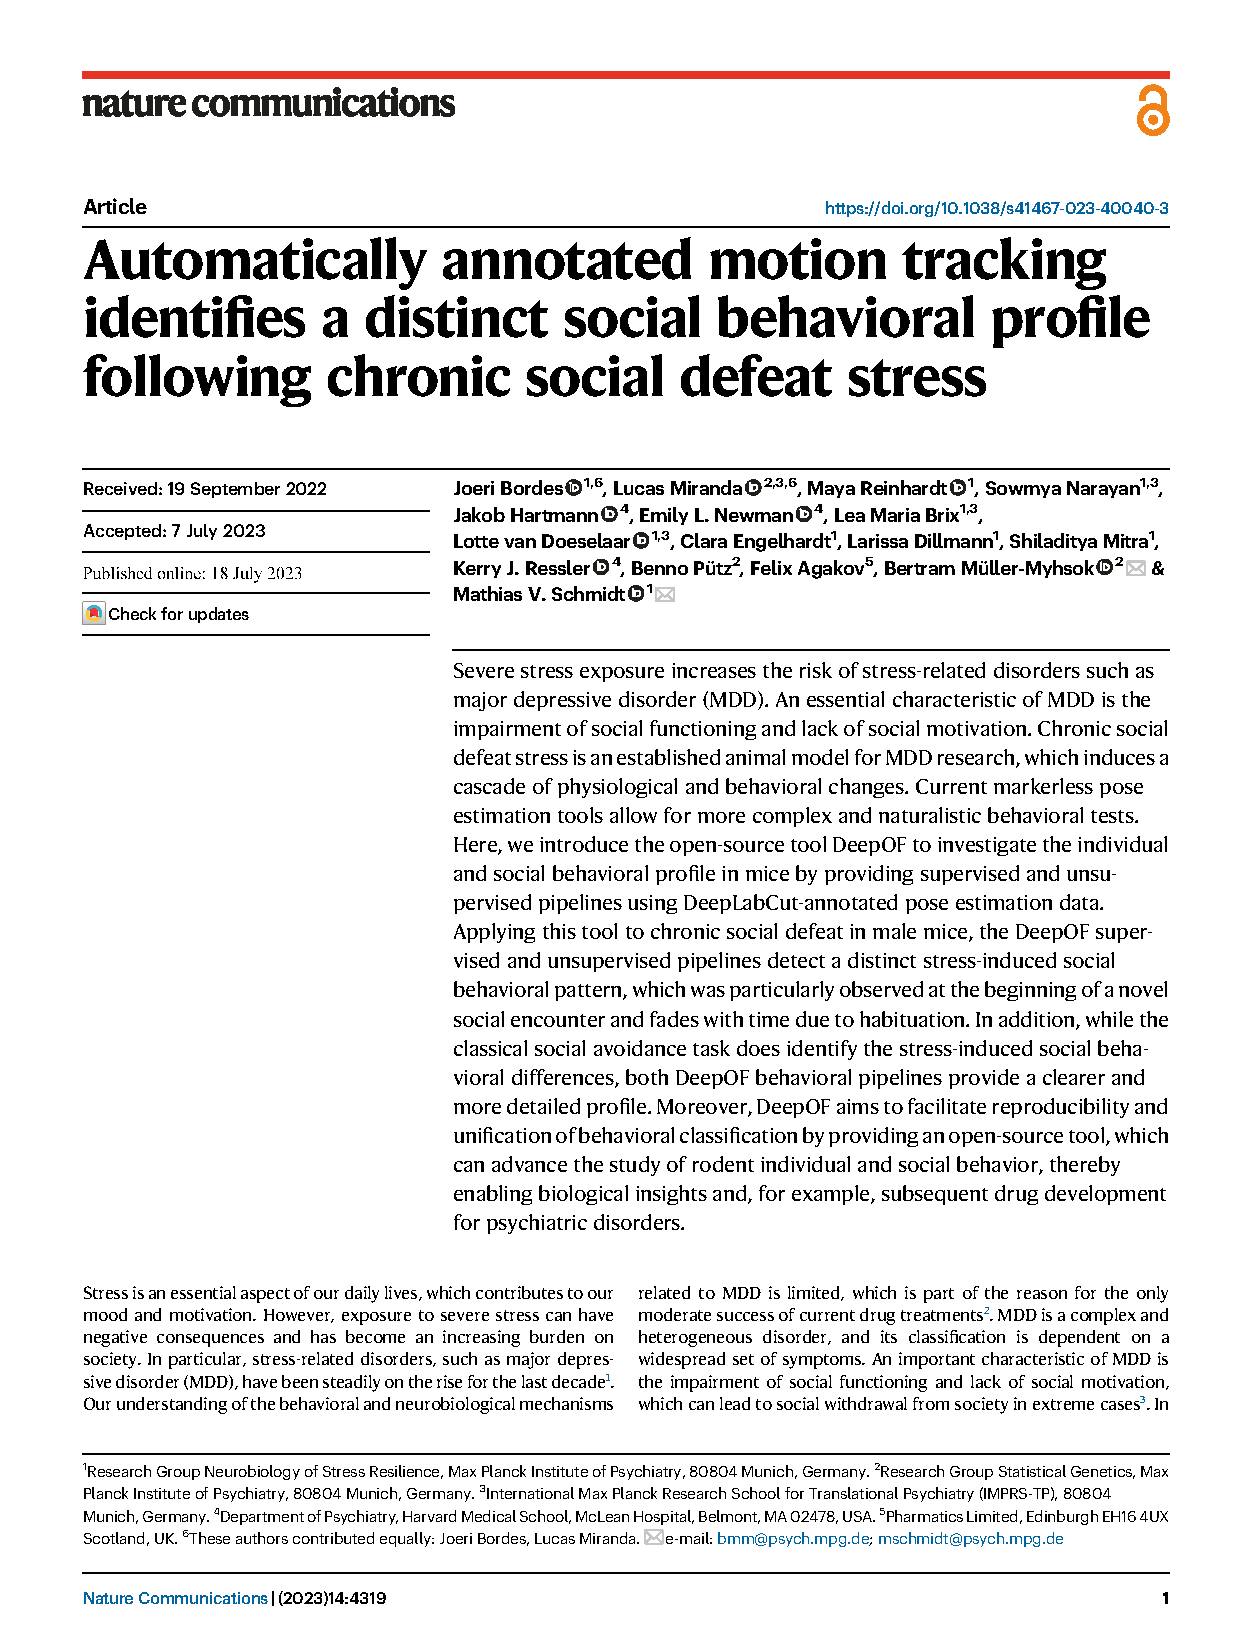
\includepdf[pages={-},
           addtolist={
           3, figure, \textbf{DeepOF workflow in detail:} an overview of data preprocessing and annotation pipelines, natcomm:fig1,
           4, figure, \textbf{Classical hallmarks for chronic social defeat stress}, natcomm:fig2,
           5, figure, \textbf{Social interaction binning yields more separable PCA projections than the social avoidance task}, natcomm:fig3,
           6, figure, \textbf{Top contributing behaviors in the social interaction task for 10 min total duration and time bins}, natcomm:fig4,
           7, figure, \textbf{Z-score correlation analysis and the exploration of susceptibility and resiliency}, natcomm:fig5,
           9, figure, \textbf{Single-animal unsupervised analyses identify different behavioral patterns between stressed and non-stressed mice during the SI task}, natcomm:fig6,
           10, figure, \textbf{SHAP analysis of unsupervised cluster assignments in the single-animal social interaction task}, natcomm:fig7
           },
           ]{Papers/natcomm.pdf}
\includepdf[pages={-},
           addtolist={
           1, figure, \textbf{Validation of rule-based annotated behaviors in DeepOF}, natcomm:supfig1,
           2, figure, \textbf{Validation of the ``stopped and huddled" classifier provided within DeepOF}, natcomm:supfig2,
           3, table, \textbf{Default thresholds used by the annotation pipeline in DeepOF}, natcomm:suptab1,
           3, table, \textbf{Datasets used in the CSDS characterization study}, natcomm:suptab2,
           4, figure, \textbf{DeepOF behavioral classifiers in the open field task}, natcomm:supfig3,
           6, figure, \textbf{DeepOF other behavioral classifiers in the social interaction task for 10 min duration}, natcomm:supfig4,
           7, figure, \textbf{Multi-animal unsupervised analyses identify different two-mice behavioral patterns between arenas containing stressed and non-stressed mice during the SI task}, natcomm:supfig5,
           9, figure, \textbf{Single-animal unsupervised analyses identify different behavioral patterns between stressed and non-stressed mice during the OF task}, natcomm:supfig6,
           11, figure, \textbf{Single-animal unsupervised analyses identify mild behavioral differences between stressed and non-stressed mice during the SA task}, natcomm:supfig7,
           12, figure, \textbf{Global single-animal embeddings across non-overlapping time bins in the SI dataset}, natcomm:supfig8,
           13, figure, \textbf{Global multi-animal embeddings across non-overlapping time bins in the SI dataset}, natcomm:supfig9,
           14, figure, \textbf{Cluster enrichment per experimental condition in the second to fourth optimal bins for the single-animal embeddings on the SI task}, natcomm:supfig10,
           15, figure, \textbf{Cluster enrichment per experimental condition in the second to fourth optimal bins reported for the multi-animal embeddings on the SI task}, natcomm:supfig11,
           16, figure, \textbf{Spatial distribution of clusters obtained using single-animal embeddings in the SI task}, natcomm:supfig12,
           17, figure, \textbf{Spatial distribution of clusters obtained using multi-animal embeddings in the SI task}, natcomm:supfig13,
           18, figure, \textbf{Spatial distribution of clusters obtained in the OF task}, natcomm:supfig14,
           19, figure, \textbf{Correlation between behavioral entropy and stress physiology Z-score}, natcomm:supfig15,
           20, figure, \textbf{SHAP analysis of unsupervised cluster assignments in the multi-animal social interaction task}, natcomm:supfig16,
           22, figure, \textbf{SHAP analysis of unsupervised cluster assignments in the open field task}, natcomm:supfig17
           },
           ]{Papers/natcomm_supplemental.pdf}

\chapter{Discussion}
\label{chap:discussion}
\section{There and back again: towards systematic quantification of natural behavior}

Understanding how living organisms (humans included), interact with and react to the environments they are exposed to has captured scientific curiosity since antiquity. As introduced in chapter \ref{chap:introduction}, modern science has come a long way since then, and a plethora of approaches have been proposed, from observational ethological studies to extremely reductionist and question-specific settings.

The advent of machine-learning-based tracking and quantification approaches is particularly exciting because it evolves in a way that is applicable across the entire board. First off, automatic quantification methods pose a unique opportunity to systematize observational studies in the wild in non-invasive ways, even without human presence. This can have tremendous impact not only in our understanding of ethology itself, but also pave the way for innovations in ecology and wildlife conservation.

Along these lines and starting broad, the current rapid decline of animal diversity (genetic, ecological, and behavioral) underscores the urgent need for tools that can conduct swift and comprehensive assessments of wildlife diversity and population dynamics \cite{Ceballos2020VertebratesExtinction}. Traditional data collection methods, which rely heavily on human fieldwork, present numerous challenges including time and cost, potential threats to wildlife and human safety, and the inevitable generation of biased datasets. These limitations significantly hinder our understanding of global ecological dynamics and the effectiveness of our conservation efforts.

However dismal the landscape may look, technological advancements show some light at the end of the tunnel. Alongside hardware breakthroughs, such as trap or on-animal cameras and automatic drones, the advancements in freely available markerless pose estimation tools presented earlier in this thesis can help in a number of ways, such as individual identification, detection of migration patterns with static sensors, injury detection, and quantification of social dynamics in the wild, to name a few \cite{Tuia2022PerspectivesConservation}.

The potential of these technologies to enhance our understanding of animal ecology, streamline conservation efforts, and even illuminate new paths for wildlife preservation is enormous. The promise they hold, coupled with their integration with machine learning, could play a significant role in turning the tide on the alarming decline in animal diversity.

Moreover, the current thesis is an example of how the opposite trend can be executed: instead of relying on artificially simplistic models that enable simple quantification in laboratory settings, richer environments can be put in place without sacrificing rigor, by leveraging markerless pose estimation and automated quantification methods.

Thus and so, and after exploring the state of the art in chapter \ref{chap:sota}, chapters \ref{chap:methods} and \ref{chap:joss} introduced a novel open-source tool, called DeepOF, capable of examining both individual and social behavioral patterns in rodents using data annotated through DeepLabCut pose estimation, in supervised and unsupervised ways. Furthermore, chapter \ref{chap:natcomm} delved into how, by applying this tool, we characterized unique individual and social behavioral profiles following CSDS, identified through traits annotated by DeepOF on C57Bl/6N subjects. Also, comparable results were obtained with our unsupervised pipeline, capable of recognizing behavioral shifts across various experimental contexts, including social interaction, single-animal open field tests, and social avoidance tasks. Furthermore, by exploring behavioral dynamics, DeepOF allowed us to systematically pinpoint how the initial moments of interaction with a new same-species partner are crucial for the social profiling of CSDS exposure in both supervised and unsupervised pipelines.

In this final chapter, we will delve into the impact that our tool can represent on the field it is immersed in, both in terms of technology development and knowledge discovery.

\section[DeepOF in context]{DeepOF in context: the current landscape of open-source software for behavioral analysis}

The release of DeepLabCut in 2018 was arguably the cornerstone of a methodological revolution in the field of behavioral neuroscience. Since then, a plethora of tools have enabled researchers not only to quickly automate previously laborious manual quantification, but to think outside the box and design more complex and naturalistic new experimental settings altogether. While empowering, the current software landscape has quickly become little short of daunting: packages for pose estimation itself \cite{Mathis2018DeepLabCut:Learning, Pereira2022SLEAP:Tracking}, supervised annotation \cite{Ro2020SimpleAnimals, Schweihoff2022A-SOiDBehavior}, unsupervised analysis \cite{Hsu2021B-SOiDBehaviors, Weinreb2023Keypoint-MoSeq:Dynamics, Luxem2022IdentifyingMotion}, and so on, propose constant innovation in a field that is still to stabilize to a new status quo, in a rapid turnover fashion that mimics the current state of other AI-dependent scenarios \cite{Shao2022TracingTrends}.
In this context, DeepOF offers the (to date) unique advantage of being an easy-to-use, label-free exploratory tool capable of annotating and analyzing motion-tracking data with just a few well-documented commands. This makes it easy for new users to adopt and try the software without big commitments, which we believe is key to success in such a rapidly changing field. Moreover, far from being a mere compilation of previously established methods, most algorithms presented are custom and adapted specifically to the tasks they are deployed to be used for. This way, easy adoption is contrasted with choice and customization, if a given user desires to take advantage of it. DeepOF is not designed to beat other available modules in their own game, but rather to act as a complement: after running an unsupervised pipeline and obtaining results that hint at particular (although non-pure) behaviors, a researcher could use the acquired knowledge to label and train supervised models using a tool like SimBA \cite{Ro2020SimpleAnimals}, for example, in order to confirm their suspicions.

Moreover, a significant advantage of DeepOF, SimBA \cite{Ro2020SimpleAnimals}, VAME \cite{Luxem2022IdentifyingMotion}, and many of the tools mentioned in this thesis is their open-source nature. Besides increasing transparency, which is always key to reproducibility, one must not forget that all these packages are being developed by (and mostly for) non-profit research organizations that thrive by interacting, debugging, and building on top of each other. This sort of synergetic, interdependent competition is a core aspect of modern science, and having access to code (including models, training schemes, and data) is crucial. Furthermore, a side effect of the overwhelming adoption of motion tracking software such as DeepLabCut is the increasing number of public datasets that are being released, which in turn enable not only the training of more powerful architectures that need less supervision \cite{Ye2022SuperAnimalBehavior}, but also the creation of open-source competitions and benchmarks. The Caltech Mouse Social Interactions (CalMS21) dataset, for example, is a pioneer in providing benchmarks for the detection of social interactions, annotation style transfer, and identification of rare traits \cite{Caltech2021TheInteractions}. Although unsupervised learning benchmarking is largely uncharted territory so far, it will be crucial to compare the DeepOF pipeline with other available methods in this area as the tools become accessible. Finally, although requiring specific hardware in many cases, such as increasingly powerful GPUs, all mentioned software is free to use, which makes it broadly accessible for research groups with limited resources. This is a huge advantage over the proprietary, often expensive, previous state-of-the-art \cite{ANY-maze}.

Moreover, several extremely recent developments introduced significant progress on foundation models for markerless, one-shot video tracking. Efforts such as TAPIR (\textit{Tracking Any Point with per-frame Initialization and temporal Refinement
}, from \textit{DeepMind}) \cite{DoerschTAPIR:Refinement} and \textit{OmniMotion} \cite{WangTrackingOnce} allow users to track any point in a given video upon labelling a single frame. While integration attempts into DeepOF have shown that tracking accuracy is yet to match DeepLabCut and other neuroscience-oriented programs, ease of use could lead to massive adoption of these pipelines as soon as models get better, with efforts in fine-tuning these general-purpose pretrained models to more specific tasks probably playing a big role in the near future.

A word of caution should be stated, however, since these models (as many others) have also increasing malicious potential if falling into the wrong hands: lightweight, powerful models for tracking and identifying individuals could be used for illegal surveillance, for example. As is currently the case in other fields, such as large language models (LLMs) \cite{Weidinger2021EthicalModels, Weidinger2022TaxonomyModels}, I believe ethical considerations need to be thoroughly taken into account when open-sourcing, especially as datasets become larger and models more capable and easier to tune.

\section{Perspectives on supervised learning on behavioral data}

Going back to the supervised pipeline provided within DeepOF, we should highlight that it offers a set of rule-based annotators and pre-trained models that free the user from the need to manually label their data. While convenient and easy to use, this approach is extremely limited to simple behaviors that can be either reduced to simple but stable rules (such as nose-to-nose contacts or climbing behaviors) or robustly generalizable across datasets (such as the huddle classifier presented in chapter \ref{chap:natcomm}).
With the increasing popularity of these tools in the research community and the aforementioned rapidly growing corpus of datasets and related competitions, it is to be expected that more complex traits will achieve similar transfer learning results in the near future. This would dramatically simplify the process of labeling and detecting specific, pre-defined behaviors, potentially eliminating the need for training new models altogether, in a fashion that would resemble the current discussion on foundation models \cite{Bommasani2021OnModels}. 

Furthermore, the current developments in Large Language Models (LLMs) and text interfaces for image processing and generation \cite{OpenAI2023GPT-4Report, Ramesh2022HierarchicalLatents} suggest that a future where describing specific, unlabeled behaviors with text to an LLM-video model capable of automatically recognizing patterns is (although far from the current state of the art) within reach, and an interesting path forward.

\section{Perspectives on unsupervised learning on behavioral data}

As introduced in chapter \ref{chap:introduction}, even if adopting a purely mechanistic definition, behavior is not inherently discrete, but arguably hierarchical. Complex actions can always be decomposed into simpler ones (typically referred to as primitives) whose repetitive nature makes them simpler to detect. Discretizing motion tracking data is therefore (as is often the case in other fields too) an ill-defined problem: with no natural solution present, a given set of clusters will focus on some aspects of behavior, leaving others behind. This renders discretization a utility problem that serves the purpose of allowing researchers to test hypotheses related to a broader scope, but which is arguably only secondary to learning robust representations.

While in DeepOF we have focused primarily on learning useful discretization models of motion, I believe future work in this direction should focus on understanding the underlying learned representations better. Along these lines, the field of representation learning has set the core principles a good and robust representation should be able to follow \cite{Le-Khac2020ContrastiveReview}. First, representations should be \textbf{expressive}, in the sense that they should be able to represent an exponential amount of configurations for their size. This would contrast, for example, with other representations such as one-hot encodings or mere hard cluster assignments. Second, good representations should be \textbf{robust} to small and local variations in input data. As an example, behavioral representations in DeepOF should vary neither with the position of the animals in the arena nor with their rotational orientation, hence these sources of variance are removed during processing. Third, good representations should be \textbf{disentangled}, meaning that learned dimensions should be uncorrelated and represent distinguishable factors with identifiable meanings. Despite not being perfect, this set of principles serves as a rule of thumb to design interpretability tests and analyses, and their usefulness in this context remains to be explored.

This type of analysis, together with the development of systematic benchmarks for unsupervised learning on motion tracking, would be an ideal framework to formally compare all the models provided within DeepOF. So far, comparisons were purely functional to choose a good default for the deployed package while exploring different variants that extended the state of the art in the field. Thus, metrics such as training time and compute resources needed, and discrimination capabilities between global animal embeddings across experimental conditions (as presented in chapter \ref{chap:natcomm}), were the main model selection criteria. The exception is the introduction of contrastive learning models, which were included in the package after the submission of the paper, and yielded comparable results with shorter training times and fewer parameters. This is exciting news moving forward and sets self-supervised alternatives as the most likely course for further immediate model development.

Thus and so, unsupervised (and self-supervised) representation learning evaluation remains, in my opinion, the most critical point for research in the immediate future. This would not only enable robust hypothesis testing and latent manipulation, but also alignment across modalities, as will be explored in the next sections.

\section{Increasing resolution in neurobiological research: behavioral quantification in context}

A living system is far more than the sum of its parts, with different biological levels interacting and regulating one another constantly in complex ways. From genetics, transcriptomics, epigenetics, and proteomics, to neural signaling, behavior, and environmental factors, being able to capture information from different biological levels in clever ways can be key to understanding any phenotype \cite{Miranda2023IncreasingBehaviors}.

Along these lines, the presented breakthroughs in motion tracking are not isolated. Recent years have seen remarkable progress in other areas relevant for neurobiological research, following a common trend of increasing experimental resolution, also outside the temporal domain \cite{Miranda2023IncreasingBehaviors}. Interestingly, in many fields other than motion tracking, breakthrough developments came mostly from the hardware side, which in turn allowed researchers to collect more data and raised the stakes of data analysis and software development in specific domains. 

As a representative example, we can explore the field of transcriptomics, where developments in single-cell resolution sequencing technologies sparked a plethora of tools and methods that innovate how data are analyzed. Here, programs like SCANPY \cite{Wolf2018SCANPY:Analysis} and SEURAT \cite{Hao2021IntegratedData} have earned recognition as the state of the art in the field, providing high-quality sets of tools, workflows, benchmarks, tutorials, and user support. They also have grown an extensive user community, which creates feedback loops with contributions and extensions which improve the software constantly. A flagrant example of such an extension is SquidPy \cite{Palla2022Squidpy:Analysis}, a package that focuses on the forefront of spatial transcriptomics,  which is greatly helping to improve our understanding of how cells in tissues are organized and interact with each other. 

All in all, this standardization offers many benefits for several connected fields (including stress research, as explored in our published commentary on STRESS \cite{Miranda2023IncreasingBehaviors}), and has a big impact not only on our basic understanding of cell makeup and gene activity in key tissues, but also on the discovery of new drug targets and development of new treatments. As a concrete example, in 2022 Lopez et al.\ used a mix of automatic behavior tracking methods and single-cell RNA-sequencing techniques to discover specific molecular patterns in different stress-related cell types, and reported a new way in which the long-lasting antidepressant effects of ketamine work in a certain type of nerve cell in a specific part of adult mice's brains \cite{Lopez2022KetamineKcnq2}. In this paper, motion tracking technology is used to automatically assess shifts in behavior across different experimental groups, illustrating how automated behavioral drug screenings can be carried out.

Moreover, transcriptomics is far from being the only case. Proteomics, for example, is being positively impacted by new developments in techniques such as mass spectrometry \cite{Mann2021ArtificialDiscovery}, and by AI-powered tools such as \textit{AlphaFold} \cite{Jumper2021HighlyAlphaFold}, which are solving biochemical problems that until a few years ago were deemed unreachable. Brain imaging and neural activity measuring are other relevant fields that have seen recent relevant advances, such as resolution improvements for functional MRI \cite{Toi2022InResolution}, and real time joint behavioral-motion capture using miniscopes and calcium sensors \cite{Dana2019High-performanceMicrocompartments, deGroot2020NinscopeInvestigations}.

As illustrated in the aforementioned paper, the combination of motion tracking quantification with many of these tools holds a lot of potential to measure the impact of genetic and biochemical changes in behavior systematically. However,  these techniques often describe different (albeit non-orthogonal) axes of the same phenomena. Although learning from and interpreting each on its own can already be useful to expand our knowledge in many ways, much information is lost in the process. 

\section{Beyond motion tracking: integrating multimodal data}

The science of learning how to better integrate these different sources of data, which can lead to a more holistic understanding of the underlying, common phenomena under study, is often referred to as \textbf{multimodal integration} (or \textbf{multimodal learning}, in the context of ML). As a side note, it is important to highlight that behavior itself is more than motion alone, and adopting a broad definition would require integrating additional variables that cannot (at least to date) be extracted from video. These include, for example, things like heart rate, respiratory rate, vocalization, and neural activity.

At a basic level, multimodal integration thus requires researchers to  draw conclusions from experiments describing multiple (complementary) axes of the same problem and drawing conclusions explaining all observed patterns. While a naïve approach may be to align the raw variables themselves (over time, for example, in the case of behavior, or as concatenated input to a model, in what is called \textbf{early integration}), there are several inherent problems that would need to be solved. For starters, different data modalities may rely on different hardware, with different collection rates, artifacts that would need to be removed, sensitivities, and overall limitations \cite{Jabeen2022ALearning}. This renders raw data alignment extremely hard, and forces researchers to often analyze modalities separately and draw joint conclusions manually. This separate processing is often called \textbf{late integration}, and while it solves many of the presented limitations, it carries the strong disadvantage of disregarding joint distributions across modalities, focusing exclusively on the marginals. When modalities are uncorrelated, however, this can be an extremely powerful framework, as illustrated by multimodal ensemble learning \cite{Ganaie2022EnsembleReview}.

Building on the previous section, the main focus of current approaches to multimodal integration deals with \textit{aligning data representations} (in what is known as \textbf{middle integration}) instead of the data themselves. By learning robust representations that extract features invariant to hardware noise and timescale nuances, these approaches hold the promise of having the best of both worlds: good alignment, while retaining and learning joint distributions. Thus and so, self-supervised approaches such as those presented in chapter~\ref{chap:methods} are showing promising results, since they allow several crucial levels of flexibility, such as having modality-specific encoders (which can deal with different types of data naturally), and specifically crafted contrastive positive and negative sampling schemes. Along these lines, the recently published package CEBRA \cite{Schneider2023LearnableAnalysis} offers a representation learning framework to learn joint embeddings using motion tracking and neural activity data with contrastive approaches. By aligning both modalities at the embedding level, CEBRA is capable of reporting non-linear neural correlates of motion, directly enabling questions regarding how one affects the other in complex ways that may be difficult to detect without computer assistance. Moreover, and in line with what was explored before in this section, two main positive and negative sampling schemes are provided: a purely unsupervised one, based on time alone and similar to that presented for DeepOF in chapter~\ref{chap:methods}, and a supervised one based on annotated labels. This makes it easier for researchers to choose between a more exploratory embedding of neural-motion interactions, or a hypothesis-driven one that can answer specific questions.

All in all, as both hardware and software technology advance, new methods are being developed that enable researchers to get a more holistic view of living organisms as systems, instead of independent collections of unrelated features. As time advances, I expect these approaches to become more prevalent and lead to better representations. While multimodal integration holds an exciting and extremely useful potential for research moving forward, however, motion tracking has the advantage of relying on relatively affordable hardware (video cameras) which enabled its wide adoption in the first place. It should thus not escape our attention that including more data modalities can be prohibitively hard, both in terms of labor intensity for data collection and elevated costs, especially in resource-constrained labs. This renders parallel efforts in representation learning on motion tracking data alone (such as DeepOF) extremely relevant too.

\section{Impact of the presented results in chronic stress research}

With the deeper understanding of the current status of behavioral analysis (and motion tracking in particular) built over the last few sections, we can now explore the impact of the presented research in our understanding of the model introduced as a case study: Chronic Social Defeat Stress.
As explored in chapters~\ref{chap:introduction} and \ref{chap:natcomm}, the individual and social behavior of animals exposed to CSDS has been extensively researched using models such as elevated plus mazes and social avoidance tasks, which can distinguish anxiety-like and altered social behaviors between cases and controls. This thesis has displayed several ways in which DeepOF has improved the state of the art in this regard, both reducing experimental effort and enabling greater analysis detail.

For starters, the observation that after exposure to the aggressive conspecific during the CSDS pipeline, experimental subjects' behavior follows an arousal pattern that fades over time due to habituation is, to the best of our knowledge, novel. The first relevant contribution of this thesis to CSDS research is then the supervised and unsupervised quantification of this arousal period, which in all our datasets was between two and two and a half minutes (and therefore close to the typical duration of a social avoidance task \cite{Kudryavtseva1991SocialStrain}). These results were moreover absent in single animal settings, which further supports this interpretation.

In line with these findings, our study showcases how the behavioral annotation provided within DeepOF leads to a more effective distinction of the social behavioral profile between stressed and non-stressed animals compared to the traditional SA task. This is a non-trivial finding: while capable of more detail, DeepOF is a general purpose tool, whereas the aforementioned task was specifically designed to detect this phenotype. I believe this is a great example of how overfitting specific measurements to our experimental designs may not always be optimal, and of how carefully tested exploratory tools can take us extremely far already.

Another result worth revisiting in this section is the differential entropy between stressed and non-stressed animals reported from our unsupervised pipeline. The fact that stressed animals display lower entropy in the discrete behaviors they explore is also non-trivial, and it highlights how reduced and focused on avoiding a potential stressor behavior becomes in stressful situations, arguably in line with the fight-or-flight response \cite{Chu2022PhysiologyReaction}.

Besides these specific contributions, DeepOF holds potential to explore in even more depth this model, such as for the identification of animals susceptible to stress and those resilient to it, which are often determined using oversimplified outcomes in the aforementioned social avoidance test, such as the fraction of time experimental animals spent close to their conspecific. While this variable (known in the literature as SA ratio) effectively distinguishes individuals affected by stress, especially in more severe CSDS conditions, our approach seems to significantly enhance the scope and sensitivity of this distinction, although more research is needed in this regard. Moreover, a tool included in DeepOF that was not put to use in this thesis and can work well in this context is the possibility to train control normative models. These work by fitting Gaussian kernel densities to the global animal embeddings of control animals, and reporting differences in the likelihood under the model between conditions. Stressed animals with embeddings that are closer to the control population could then be tagged as resilient. The next and final section on translational research applications will further explore this idea, showcasing its potential for more complex settings, such as the detection of the depression-like syndrome presented in chapter \ref{chap:introduction}.

In conclusion, the annotation pipelines implemented in DeepOF provide a more comprehensive and precise individual and social behavioral profile of animals exposed to CSDS when compared to the previous state of the art in the field. This has several implications moving forward, such as the potential adoption of DeepOF (or similar tools) for CSDS quantification as a standard procedure, and the deeper exploration of the tool for other aspects not discussed here. Moreover, an important factor contributing to the overall success of DeepOF in the presented social behavioral profiling lies in its experimental setup. While the social avoidance task relies on confined animals (typically in wired mesh cages, which prevent natural interaction between freely moving animals), open field settings allow for a much more natural interaction. Moreover, in the SA task, confined animals may display anxiety-related behaviors that influence their physiological state and their social interaction and approach behaviors with the conspecific.

Finally, and while we believe that our contributions to CSDS are significant and worth mentioning, we should not lose sight of the broader scope. Chronic stress is just one example setting in which such pipeline can be applied, and much more remains to be explored in other equivalent or more complex models. The next and final section will explore this in detail, focusing on how translational research can be positively affected with tools such as these.


\section{Frontiers of the field: between translational research and knowledge discovery}

As thoroughly explored in chapter \ref{chap:introduction}, the current state of research in applied neurobiology and psychiatry research lies far from the clinic. While many studies present innovations in drug development, genetic markers, and more, little is translated to real patients, in a phenomenon that has been described as the translational gap \cite{Shemesh2023ANeuroethology}. Moreover, despite animal models being adopted decades ago, their use to mimic mental disorders hasn’t managed to live up to the expectations. This is due to many reasons, such as the complexity of mental disorders per se and their prominent environmental causes, which are to date difficult to replicate in animals \cite{vonMucke-Heim2022IntroducingMice}. On top of this, and the lack of biologically-driven definitions of mental disorders makes the problem harder, as currently described entities could correspond to more than one etiologically relevant entity \cite{Miranda2021SystematicSubtyping}.

Even when taking all these issues into account, I believe there is light at the end of the tunnel, and that the potential of modern behavioral quantification in this regard is significant. Firstly, because it allows for finer-grain measurements that can be used to get more disentangled and data-driven definitions of the diseases under study, as seen with the RDoC initiative \cite{Vilar2019TranslationalRDoC}. Second, because once these definitions are agreed upon, this technology could simplify the accurate assignment of labels to subjects under study, decreasing the focus on more subjective measurements \cite{Miranda2021SystematicSubtyping}. Moreover, as seen with the depression-like syndrome introduced in chapter \ref{chap:introduction}, these disentangled definitions are key to improving back-translation \cite{vonMucke-Heim2022IntroducingMice}. That is, the definition of human-equivalent diseases in animal models that are as close as possible to the clinically relevant phenotype. In this regard, the normative modelling pipeline introduced in the previous section can play a key role: as a follow-up study to what was presented in chapter \ref{chap:natcomm}, we are currently using DeepOF to build domain specific normative models for DLS. This way, animals can be scored on each behavioral domain that escapes the species barrier (which are \textit{loss of energy and fatigue}, \textit{lack of concentration and indecisiveness}, \textit{psychomotor agitation or retardation}, \textit{disturbed sleep with hyper or hyposomnia}, \textit{apetite or weight changes}, and \textit{diminished interest or pleasure in activities}). By detecting shifts on each of these domains, many of which are carried out with DeepOF, we can get individual profiles for each experimental mouse. This way, DeepOF can be used in two stages, first to select individuals that meet stricter inclusion criteria for follow-up studies, and second to detect shifts in behavior upon applying a treatment (such as a drug).

Moreover, these technologies are not limited to animal models. Given that the ultimate goal of clinical research is to comprehend and enhance the quality of life for humans, assigning humans to the correct labels, and study their shifts in behavior systematically, is also crucial. In this context, advancements in comprehending human behavior through virtual reality (VR) are noteworthy. Presently, VR enables researchers to accurately monitor movement in meticulously designed settings, facilitating the transfer of paradigms like fear conditioning to human participants noninvasively \cite{Binder2022FacingPhobia, Rubio2023Auto-EncodersPerspectives}. Tools such as DeepOF can be applied to this type of data as well \cite{Sahili2023Spatio-TemporalSurvey}.

Finally, and while translation to the clinic is set as the final goal in this context, these technologies can also be of great help to acquire new knowledge. For example, the use of unsupervised learning in motion tracking data has the potential to uncover new behaviors that are systematically expressed in certain conditions, although more research in novel situations is needed in this regard \cite{Mathis2020APerspectives}. Moreover, detecting unsupervised shifts in behavior can be of great use in many high-throughput and hypothesis-free situations, such as Quantitative Trait Loci (QTL) mapping \cite{Abiola2003TheView}. This refers to a statistical method that aims to link two types of information, namely phenotypic data (quantitative traits, as behavior in this case) and genotypic data in the cohorts under study. This way, researchers can identify regions in the genome that can influence the variation of a given trait.

Even though in the context of DeepOF and similar tools these quantitative traits could be any measured parameter (such as speed, locomotion, social interactions, etc.), I believe the unsupervised animal embeddings introduced earlier are the most interesting opportunity in this regard. By detecting global shifts in behavior that are not associated with any particular hypothesis, researchers can increase throughput and scope massively. Moreover, detected shifts can then be analyzed individually, to dissect the differentially expressed patterns in a hypothesis-driven manner with the same tool. A similar idea is already being applied (although relying on supervised learning models detecting specific traits) for high-throughput drug discovery \cite{IndustrializingDiscovery}.

Linking together everything discussed in this section, DeepOF and similar tools are already being used today to revolutionize research in animal and human behavior, and hold increasing potential to have a positive impact on the current definitions of psychiatric conditions, improve pre-clinical and clinical trials, and aid relevant biological and drug discovery. The future of the field looks increasingly promising, and our contribution is but a grain of sand.

\chapter{Conclusion \& Outlook}
\label{chap:conclusions}
This thesis delved into the state of the art of animal motion tracking using key point estimation, and its further analysis using different annotation approaches. Three main goals were defined, including the implementation of novel deep clustering algorithms for the unsupervised analysis of motion tracking data, their deployment alongside other tools as part of a Python package, and their application to characterize a real-world behavioral model.

Along these lines, chapter~\ref{chap:introduction} introduced the broad topics under discussion, including definitions of behavior, history of its quantification and application, and chronic stress as a case study. Moreover, it explored the broad technical foundations for what the thesis aimed to present. 

Chapter~\ref{chap:sota} explored the technical aspects of behavioral analysis in more detail and presented state-of-the-art tools to analyze motion-tracking data in both supervised and unsupervised ways. 

Subsequently, chapter~\ref{chap:methods} explored the methodological aspects of the newly introduced algorithms, and all analyses that were carried out for the presented results. 

Chapter~\ref{chap:joss} then moved to introduce DeepOF, our novel Python package, as published in the Journal of Open Source Software (JOSS). This paper, although short, serves as an entry point to the DeepOF ecosystem, its documentation, and contribution guidelines. Moreover, this publication included a code peer-review process of vital importance to what this thesis aims to stand for: open science, both in terms of methods and code. We believe this small paper is an important milestone for our vision of what DeepOF and similar tools represent in the field. 

Next, chapter~\ref{chap:natcomm} demonstrated how the developed tools can be applied to a real world animal model, such as Chronic Social Defeat Stress. This set of results, published in Nature Communications, explores both supervised and unsupervised pipelines included, and how they yield overlapping yet complementary insights into the shifts in behavior that chronic stress causes in male laboratory mice. We hope this is but a kick-start example of what can be accomplished with this tool, and expect to gain insight into other animal models in the future, both with experiments carried out by direct colleagues and external users.

Finally, chapter~\ref{chap:discussion} attempts to put the presented developments in context, delving into the potential impact of the provided tools in several related fields, such as ecology, integration with other data modalities, and QTL discovery. Moreover, a perspective on how the field is likely to evolve in the near future is discussed.

All in all, the current thesis is but an example of an evolving field, in which (as in many other areas currently powered by machine learning) novel tools are enabling both automation and discovery in ways that were not thought possible a decade ago. When putting these developments in context and as both technology and biological knowledge progress, from single cells to social behavior \cite{Miranda2023IncreasingBehaviors}, the dream of jointly mapping behavioral responses to stimuli in a holistic manner is closer than ever.

%-------------------------------------------------------------------------------
% Bibliography
%-------------------------------------------------------------------------------
%\backmatter
% unsrturl-custom works only with hyperref loaded
% use other styles like unsrt when hyperref is not loaded
\bibliographystyle{unsrturl-custom}
\bibliography{bibliography}

\nocitePhD{*}
\bibliographystylePhD{unsrturl-custom}
\bibliographyPhD{phd_bibliography}

\end{document}

%%% Local Variables:
%%% mode: latex
%%% TeX-master: t
%%% End:
